%!TEX root=./LIVRO.tex
\chapter[O alfabeto, as vogais e as consoantes]{\Large O alfabeto, as vogais e as consoantes}
\markboth{Módulo 1}{}

\colorsec{Habilidade do SAEB}

\begin{itemize}
\item Relacionar elementos sonoros das palavras com sua representação escrita.
\end{itemize}

\colorsec{Habilidade da BNCC}

\begin{itemize}
\item EF02LP03.
\end{itemize}

Para escrever as palavras, usamos as \textbf{letras}. 
Juntas, elas compõem o \textbf{alfabeto}, que é formado por 26 letras. 

As \textbf{vogais} são \textit{a, e, i, o, u}, e as outras letras são
chamadas de \textbf{consoantes}. Veja:

\begin{center}
\textsc{b c d f g h j k l m n p q r s t v w x y z}\hfill
\end{center}

Cada letra possui um nome e um som, que, quando estão juntos, podem
formar muitas palavras.

\begin{longtable}[]{@{}llllll@{}}
\toprule
\textsc{Pato} & \textsc{Vaca} & \textsc{Bola} & \textsc{Tatu} &
\textsc{Fada} & \textsc{Doce}\tabularnewline
\bottomrule
\end{longtable}

A letra C pode apresentar dois sons diferentes de acordo com a vogal que
acompanha. Por exemplo: junto com as vogais A, O e U, apresenta o som de 
/k/; junto com E e I apresenta o som de /s/.
 
%Felipe: precisamos padronizar como vamos grafar as letras e os fonemas, como ocorreu na frase acima. (Rogério, 13/3/23, 14h31)

Algumas palavras com o som de /k/ também podem ser escritas com Q,
mas vale lembrar que o Q vem sempre acompanhado de U e de mais uma
vogal, e é esta última vogal que vai marcar o som da sílaba. Observe:

\begin{center}

\begin{table}[hb!]
\begin{tabular}{|ccc|}
\hline
\multicolumn{3}{|l|}{\textbf{Palavras c com som de /k/}} \\ \hline
\multicolumn{1}{|c|}{cuca} & \multicolumn{1}{c|}{casa} & coco \\ \hline
\multicolumn{3}{|l|}{\textbf{Palavras c com som de /s/}} \\ \hline
\multicolumn{1}{|c|}{cebola} & \multicolumn{1}{c|}{cinco} & cisne \\ \hline
\multicolumn{3}{|c|}{\textbf{Palavras com qu}} \\ \hline
\multicolumn{1}{|c|}{queijo} & \multicolumn{1}{c|}{quilo} & quero \\ \hline
\end{tabular}
\end{table}

\end{center}

Veja a grafia dessas palavras.

TATU GALO 

Na grafia das palavras com as vogais O e U, o O no final de palavras é
fraco, e o U é sempre forte.

A letra /k/ é usada apenas em situações como nomes de
pessoas, como Kátia, e palavras estrangeiras como
\textit{ketchup, kit, kibon} e \textit{kaiser}.

%\pagebreak

\colorsec{Atividades}

\num{1} Complete os nomes das figuras com as letras que estão faltando.

\begin{figure}[htpb!]
\begin{center}
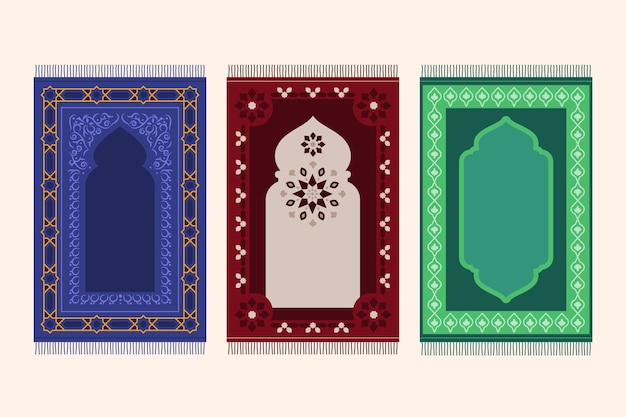
\includegraphics[width=.5\textwidth]{media/image1.jpeg}
\end{center}
\end{figure}

\begin{center}
T \reduline{A} P \reduline{E} T \reduline{E}
\end{center}

\begin{figure}[htpb!]
\begin{center}
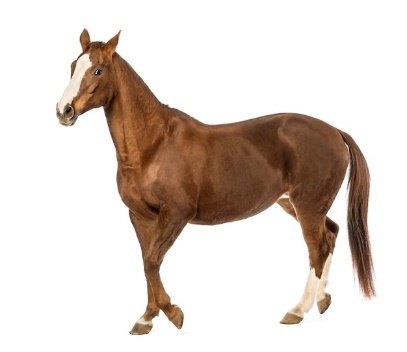
\includegraphics[width=.4\textwidth]{media/image2.jpeg}
\end{center}
\end{figure}

\begin{center}
\textbf{\textsc{ C \reduline{A} V \reduline{A} L \reduline{O}}}
\end{center}

\pagebreak

\begin{figure}[htpb!]

\includegraphics[width=.5\textwidth]{media/image3.jpeg}
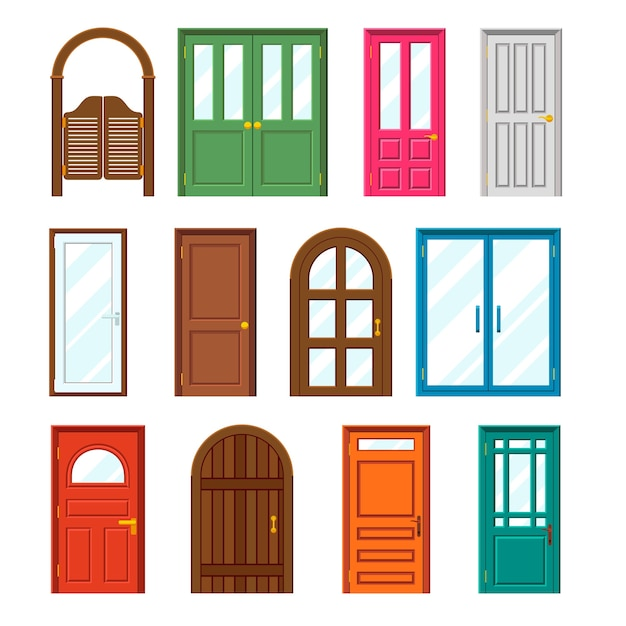
\includegraphics[width=.5\textwidth]{media/image4.jpeg}
\end{figure}

\reduline{E} STR \reduline{E} L \reduline{A} \hspace{6cm} P \reduline{O} RT \reduline{A}

Você completou as palavras com

\begin{boxlist}
\boxitem{\white{X}} Vogais 

\boxitem{\white{X}} Consoantes
\end{boxlist}

%\coment{Apresente as vogais em cartaz. Pergunte o nome dos objetos representados nas imagens e, em seguida, convide as crianças para montar as palavras no alfabeto móvel para identificar as letras faltantes.}

\num{2} Complete o alfabeto com as letras que estão faltado.

\begin{center}
\Large
\begin{tabular}{|l|l|llllll}
\hline
\textbf{A} & \rosa{B} & \multicolumn{1}{l|}{\rosa{C}} & \multicolumn{1}{l|}{\rosa{D}} & \multicolumn{1}{l|}{\textbf{E}} & \multicolumn{1}{l|}{\rosa{F}} & \multicolumn{1}{l|}{\rosa{G}} & \multicolumn{1}{l|}{\rosa{H}} \\ \hline
\textbf{I} & \rosa{J} & \multicolumn{1}{l|}{\rosa{K}} & \multicolumn{1}{l|}{\rosa{L}} & \multicolumn{1}{l|}{\rosa{M}} & \multicolumn{1}{l|}{\rosa{N}} & \multicolumn{1}{l|}{\textbf{O}} & \multicolumn{1}{l|}{\rosa{P}} \\ \hline
\rosa{Q} & \rosa{R} & \multicolumn{1}{l|}{\rosa{S}} & \multicolumn{1}{l|}{\rosa{T}} & \multicolumn{1}{l|}{\textbf{U}} & \multicolumn{1}{l|}{\rosa{V}} & \multicolumn{1}{l|}{\rosa{W}} & \multicolumn{1}{l|}{\rosa{X}} \\ \hline
\rosa{Y} & \rosa{Z} & \textbf{} & \textbf{} & \textbf{} & \textbf{} & \textbf{} & \textbf{} \\ \cline{1-2}
\end{tabular}
\end{center}

Você completou os quadradinhos com:

\begin{boxlist}
\boxitem{\white{X}} Vogais 

\boxitem{\white{X}} Consoantes
\end{boxlist}

%\coment{Leve o alfabeto móvel para sala e convide os alunos para organizar as letras na ordem certa. Em seguida, oriente-os a preencher o quadro; depois ajude a separar vogais e consoantes.}

\num{3} Leia o poema.

\textbf{A vaca Filomena e a formiga Violeta}


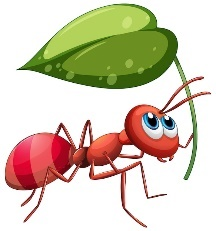
\includegraphics[width=.2\textwidth]{media/image5.jpeg}
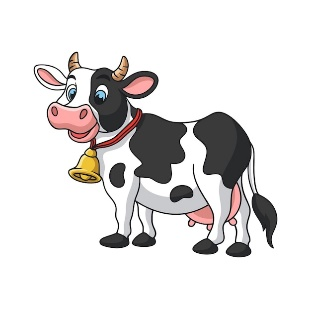
\includegraphics[width=.3\textwidth]{media/image6.jpeg}

\begin{verse}
A vaca Filomena\\
mora na vila formosa.\\
A formiga Violeta\\
mora na cerca cor de rosa.

A vaca Filomena\\
come as uvas da parreira.\\
A formiga Violeta\\
acha isto uma besteira.
\end{verse}

\fonte{Isabel Cristina Silveira Soares. https://seceducacao.padua.rj.gov.br/wp-content/uploads/2021/05/3o-ano-Ling.-Portuguesa-ATIV.17.pdf.
Acesso 28 de Fev 2023.}

Encontre e pinte no texto todas as palavras iniciadas com F e V. 
Depois escreva abaixo as palavras que encontrou.

\reduline{As palavras encontradas são as seguintes: vaca, Filomena, vila,
formosa, formiga, violeta.
Leve as palavras \textit{vaca} e \textit{formiga} em uma caixinha e
apresente-as para as crianças. Faça a leitura das palavras e estimule 
questionamentos sobre esses animais: os alunos sabem como eles são?
Onde esses animais vivem? Que sons eles emitem? Faça com os
alunos a leitura do poema e oriente a localização das palavras iniciadas
com as consoantes V e F.\hfill}

\num{4} Complete os espaços a seguir com as letras iniciais das palavras
\textit{violeta} e \textit{filomena}.

%\coment{Leve as palavras Violeta e Filomena em um cartaz. Explore a letra inicial e o som da letra nas palavras.}

\begin{figure}[htpb!]

\includegraphics[width=.3\textwidth]{media/image7.jpeg}
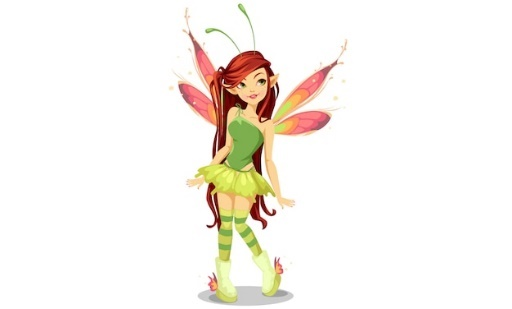
\includegraphics[width=.3\textwidth]{media/image8.jpeg}
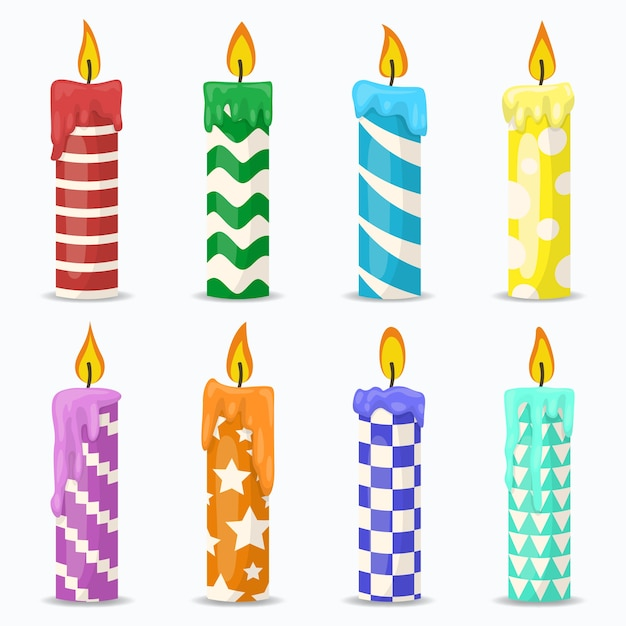
\includegraphics[width=.3\textwidth]{media/image9.jpeg}
\end{figure}

\reduline{F} ACA \hspace{4cm} \reduline{F} ADA \hspace{3cm} \reduline{V} ELA

\pagebreak
\begin{figure}[htpb!]
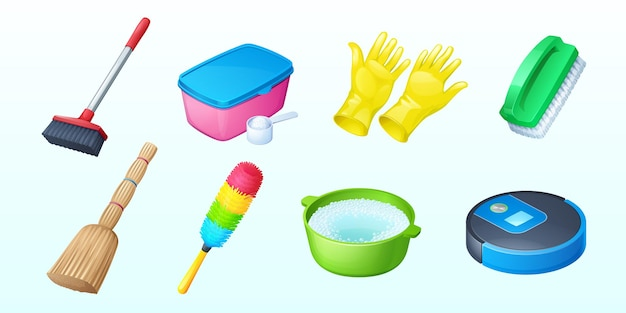
\includegraphics[width=.3\textwidth]{media/image10.jpeg}
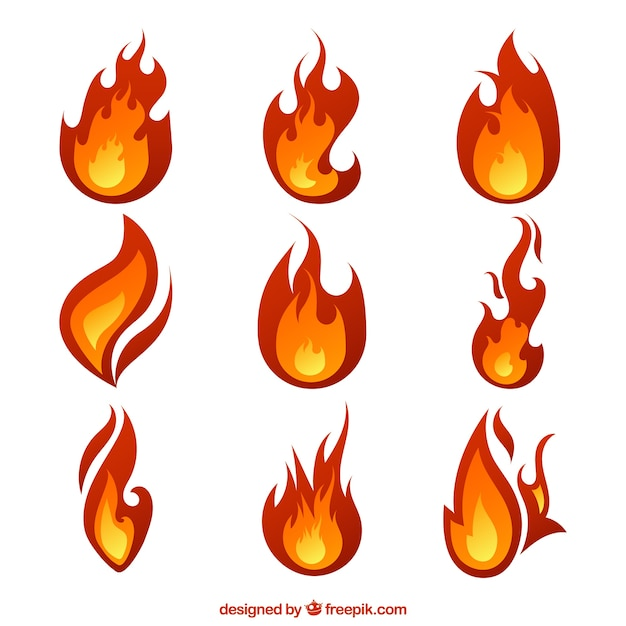
\includegraphics[width=.3\textwidth]{media/image11.jpeg}
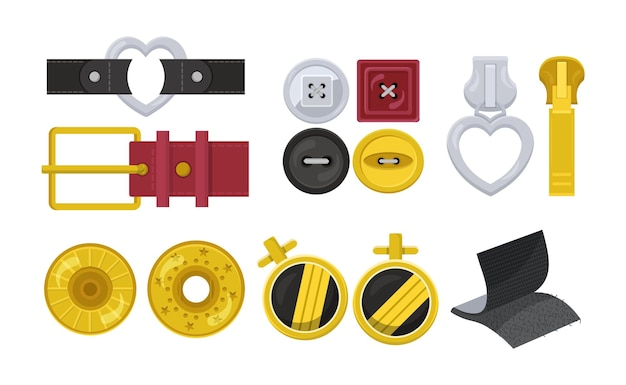
\includegraphics[width=.3\textwidth]{media/image12.jpeg}
\end{figure}

 \reduline{V} ASSOURA \hspace{4cm} \reduline{F} OGO \hspace{3cm} \reduline{F} IVELA

\begin{figure}[htpb!]
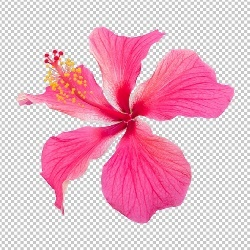
\includegraphics[width=.3\textwidth]{media/image13.jpeg}
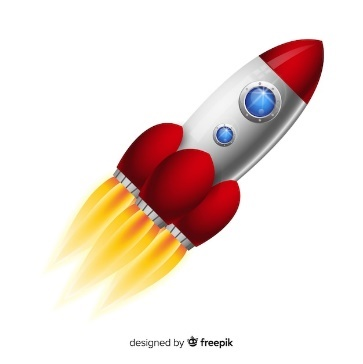
\includegraphics[width=.3\textwidth]{media/image14.jpeg}
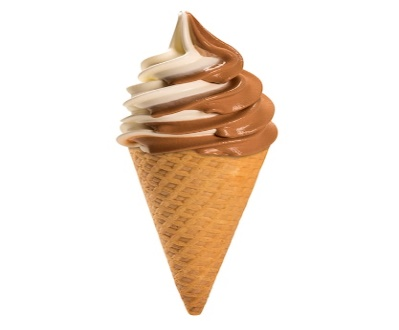
\includegraphics[width=.3\textwidth]{media/image15.jpeg}
\end{figure}

\reduline{F} LOR \hspace{4cm} \reduline{F} OGUETE \hspace{3cm} SOR \reduline{V} ETE


\num{5} Pinte as iniciais de cada palavra.

%\coment{Leve para sala palavras iniciadas pelas letras T, D, F, V, B, P. Convide as crianças para fazer a leitura, identificado o som das letras iniciais e finais, e quantidade de sílabas. Também é possível trabalhar a função social da escrita das palavras}.

\begin{center}
\begin{tabular}{|c|c|c|c|c|}
\hline
\textbf{VACINA} & F & T & D & \rosa{V} \\ \hline
\textbf{TESOURA} & P & D & \rosa{T} & F \\ \hline
\textbf{VASSOURA} & B & T & \rosa{V} & F \\ \hline
\textbf{FACA} & V & \rosa{F} & D & T \\ \hline
\textbf{DEDO} & T & V & F & \rosa{D} \\ \hline
\textbf{PANELA} & V & T & \rosa{P} & B \\ \hline
\textbf{DOMINÓ} & B & \rosa{D} & T & P \\ \hline
\textbf{BONECA} & F & P & \rosa{B} & D \\ \hline
\end{tabular}
\end{center}

\pagebreak
\num{6} Numere os desenhos conforme os números das palavras.

%\coment{Faça leitura das palavras com as crianças, de modo que elas identifiquem a numeração e façam a associação correta.}

\begin{multicols}{3}
\begin{enumerate}
\item BOLA

\item FOCA

\item TATU

\item PANELA

\item TAPETE

\item FORMIGA

\item DADO

\item VACA

\item PATO

\item BONECA
\end{enumerate}
\end{multicols}

\begin{longtable}[]{@{}llll@{}}
\reduline{\_\_10\_\_} &
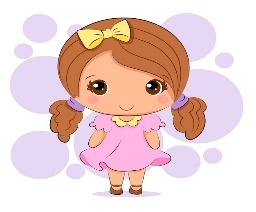
\includegraphics[width=1.16667in,height=0.96319in]{media/image16.jpeg} &
\reduline{\_\_8\_\_} &
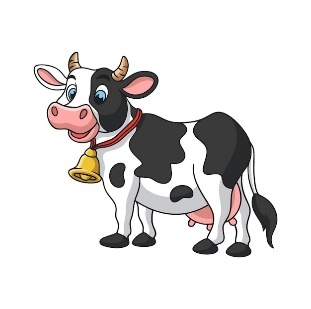
\includegraphics[width=1.16127in,height=0.95833in]{media/image17.jpeg}\tabularnewline
\reduline{\_\_2\_\_} &
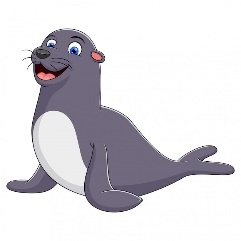
\includegraphics[width=1.09375in,height=1.09375in]{media/image18.jpeg} &
\reduline{\_\_4\_\_} &
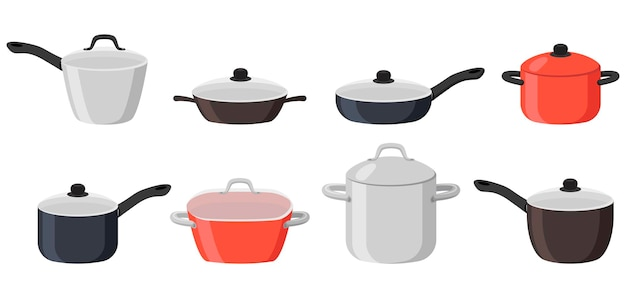
\includegraphics[width=1.27986in,height=0.98958in]{media/image19.jpeg}\tabularnewline
\reduline{\_\_3\_\_} &
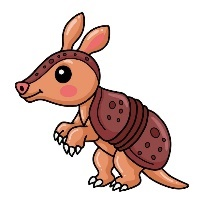
\includegraphics[width=0.92708in,height=0.92708in]{media/image20.jpeg} &
\reduline{\_\_6\_\_} &
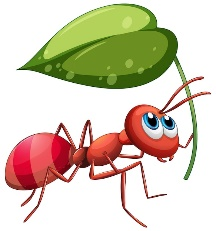
\includegraphics[width=0.97986in,height=1.05208in]{media/image21.jpeg}\tabularnewline
\reduline{\_\_1\_\_} &
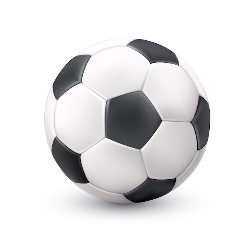
\includegraphics[width=1.13542in,height=1.13542in]{media/image22.jpeg} &
\reduline{\_\_7\_\_} &
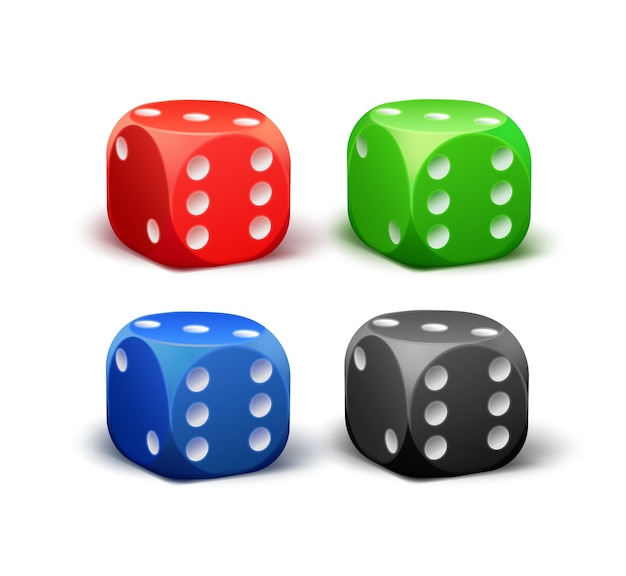
\includegraphics[width=1.23958in,height=1.15833in]{media/image23.jpeg}\tabularnewline
\reduline{\_\_9\_\_} &
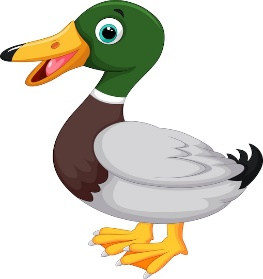
\includegraphics[width=1.19722in,height=1.27083in]{media/image24.jpeg} &
\reduline{\_\_5\_\_} &
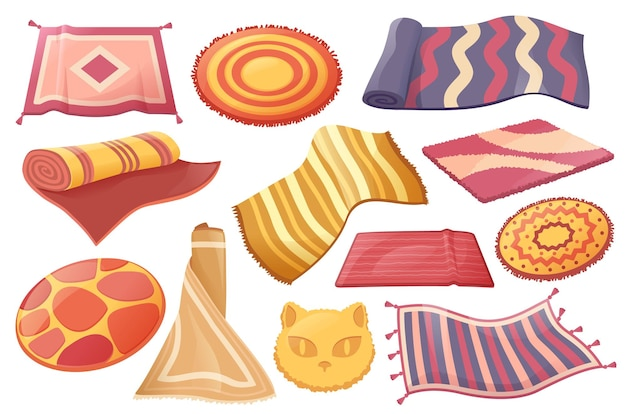
\includegraphics[width=2.21875in,height=1.11458in]{media/image25.jpeg}\tabularnewline
\end{longtable}

\pagebreak
\num{7} Complete as palvaras com \textbf{-ca -co -cu} ou \textbf{-qua -que -qui}.

%\coment{Convide as crianças a falar o nome das imagens para identificar a grafia da palavra.}

\begin{figure}[htpb!]

\includegraphics[width=.24\textwidth]{media/image26.jpeg}
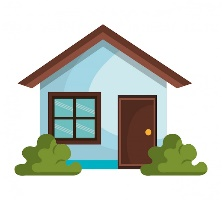
\includegraphics[width=.24\textwidth]{media/image27.jpeg}
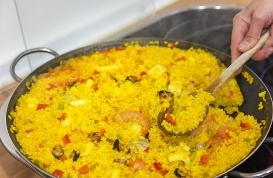
\includegraphics[width=.24\textwidth]{media/image28.jpeg}
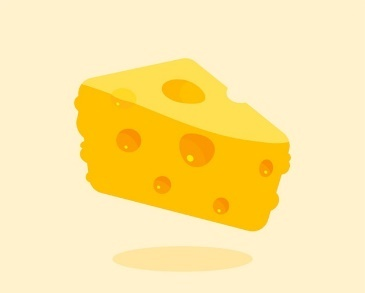
\includegraphics[width=.24\textwidth]{media/image29.jpeg}
\end{figure}

\reduline{CU} TIA \hspace{2cm} \reduline{CA} SA \hspace{2cm} \reduline{CU} SCUZ \hspace{2cm} \reduline{QUE} IJO

\begin{figure}[htpb!]
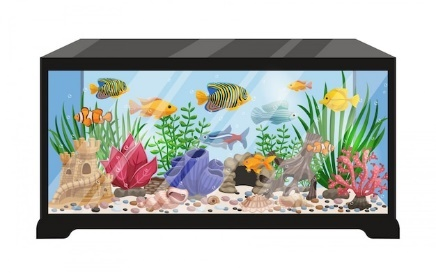
\includegraphics[width=.24\textwidth]{media/image30.jpeg}
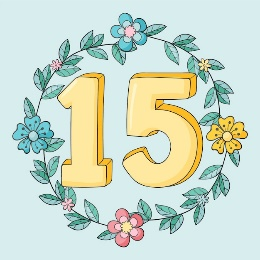
\includegraphics[width=.24\textwidth]{media/image31.jpeg}
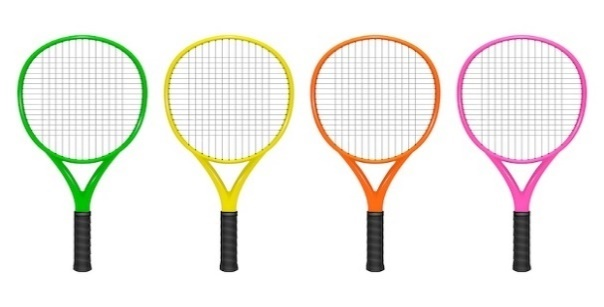
\includegraphics[width=.24\textwidth]{media/image32.jpeg}
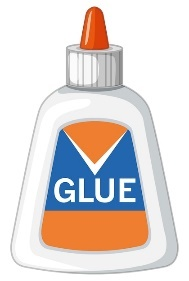
\includegraphics[width=.24\textwidth]{media/image33.jpeg}
\end{figure}

A \reduline{QUÁ} RIO \hspace{1cm} \reduline{QUI} NZE \hspace{1cm} RA \reduline{QUE} TE \hspace{1cm} \reduline{CO} LA


\num{8} Encontre a sílaba mais forte e complete com O ou U.

%\coment{Leve para a classe uma caixinha enfeitada com palavras terminadas com O e U. Passe a caixinha para os alunos em círculo, ao som de uma música. Quando a música parar, o aluno que estiver com a caixinha na mão deve ler a palavra observando a letra  final. Em seguida, convide toda a turma a pronunciar a palavra e, então, descobrir a sílaba forte. Explique como descobrir quando a sílaba é forte e fraca, ensinando que, quando o U está no final, ele é sempre forte, e que o O é sempre fraco no final das palavras.}

\begin{figure}[htpb!]
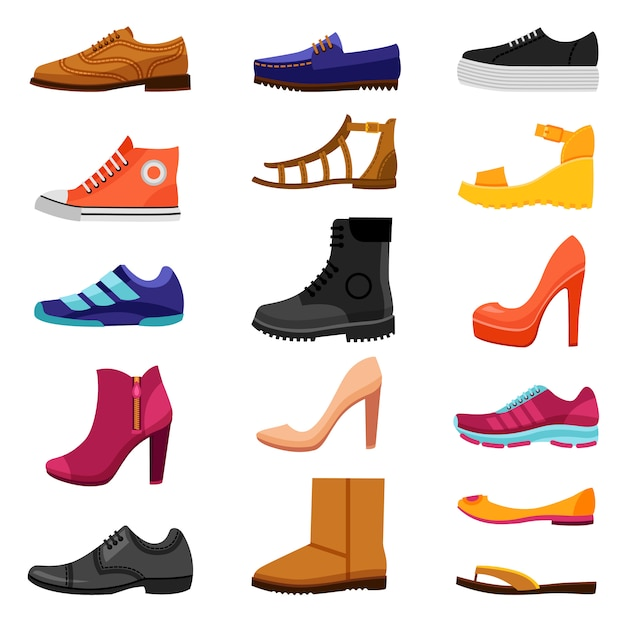
\includegraphics[width=.3\textwidth]{media/image34.jpeg}
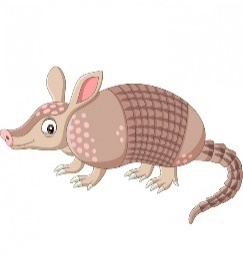
\includegraphics[width=.3\textwidth]{media/image35.jpeg}
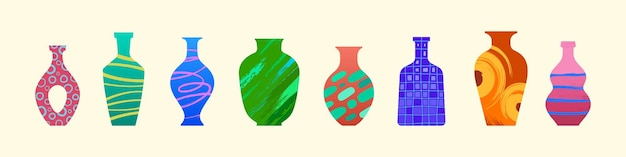
\includegraphics[width=.2\textwidth]{media/image36.jpeg}
\end{figure}

SAPAT \reduline{O} \hspace{3cm} VAS \reduline{O} \hspace{2cm} TAT \reduline{U}

\begin{figure}[htpb!]
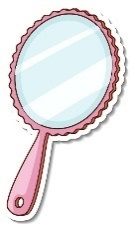
\includegraphics[width=.2\textwidth]{media/image37.jpeg}
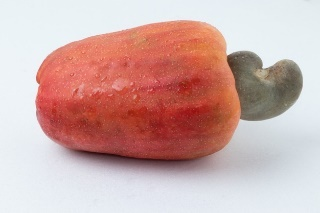
\includegraphics[width=.3\textwidth]{media/image38.jpeg}
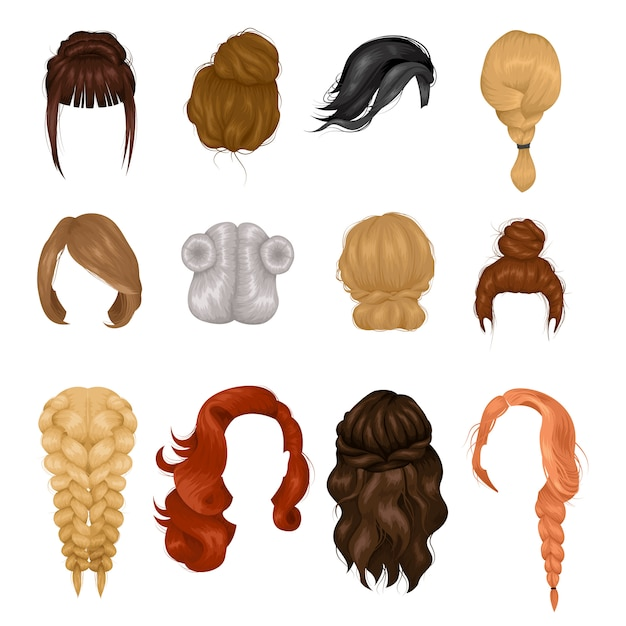
\includegraphics[width=.2\textwidth]{media/image39.jpeg}
\end{figure}

ESPELH \reduline{O} \hspace{1cm} CAJ \reduline{U} \hspace{2cm} CABEL \reduline{O}


\num{9} Pinte as palvras escritas com C que tem o som de S.
%Felipe: aqui precisamos padronizar, como comentei anteriormente. 

%\coment{Leve para sala palavras escritas com C. Organize uma roda de conversa na qual você orientará os alunos a organizar as palavras de acordo com a vogal que acompanha a letra C. Em seguida, explique a regra para descobrir se o C tem som de K ou S.}

\begin{longtable}[]{@{}lllll@{}}
\toprule
\textbf{CINEMA} & \textbf{CASA} & \textbf{CISNE} & \textbf{CEGO} &
\textbf{COCADA}\tabularnewline
\midrule
\endhead
\textbf{CADEIRA} & \textbf{CARRO} & \textbf{CINTO } & \textbf{COCO} &
\textbf{CAMA}\tabularnewline
\bottomrule
\end{longtable}

\num{10} Troque as letras e forme outras palavras.

%\coment{Utilize o alfabeto móvel com as palavras solicitadas no exercício e outras. Também é possível fazer a brincadeira da forca.}

\begin{longtable}[]{@{}lll@{}}
\toprule
\textbf{V POR F} & \textbf{D POR T} & \textbf{B POR P}\tabularnewline
\midrule
\endhead
\textbf{VACA} & \textbf{DADO} & \textbf{BODE}\tabularnewline
\textbf{\reduline{F}ACA} & \textbf{\reduline{T}ATO} & \textbf{\reduline{P}ODE}\tabularnewline
\textbf{VILA} & \textbf{DIA} & \textbf{BOTE}\tabularnewline
\textbf{\reduline{F}I LA} & \textbf{\reduline{T}IA} & \textbf{\reduline{P}OTE}\tabularnewline
\bottomrule
\end{longtable}

\pagebreak
\num{11} Complete a cruzadinha com o nome das figuras.

%\coment{Explore as frutas e legumes da atividade, fazendo questionamentos. Monte as palavras no alfabeto móvel com as crianças. Em seguida, oriente a escrita na cruzadinha.}

\begin{figure}[htpb!]
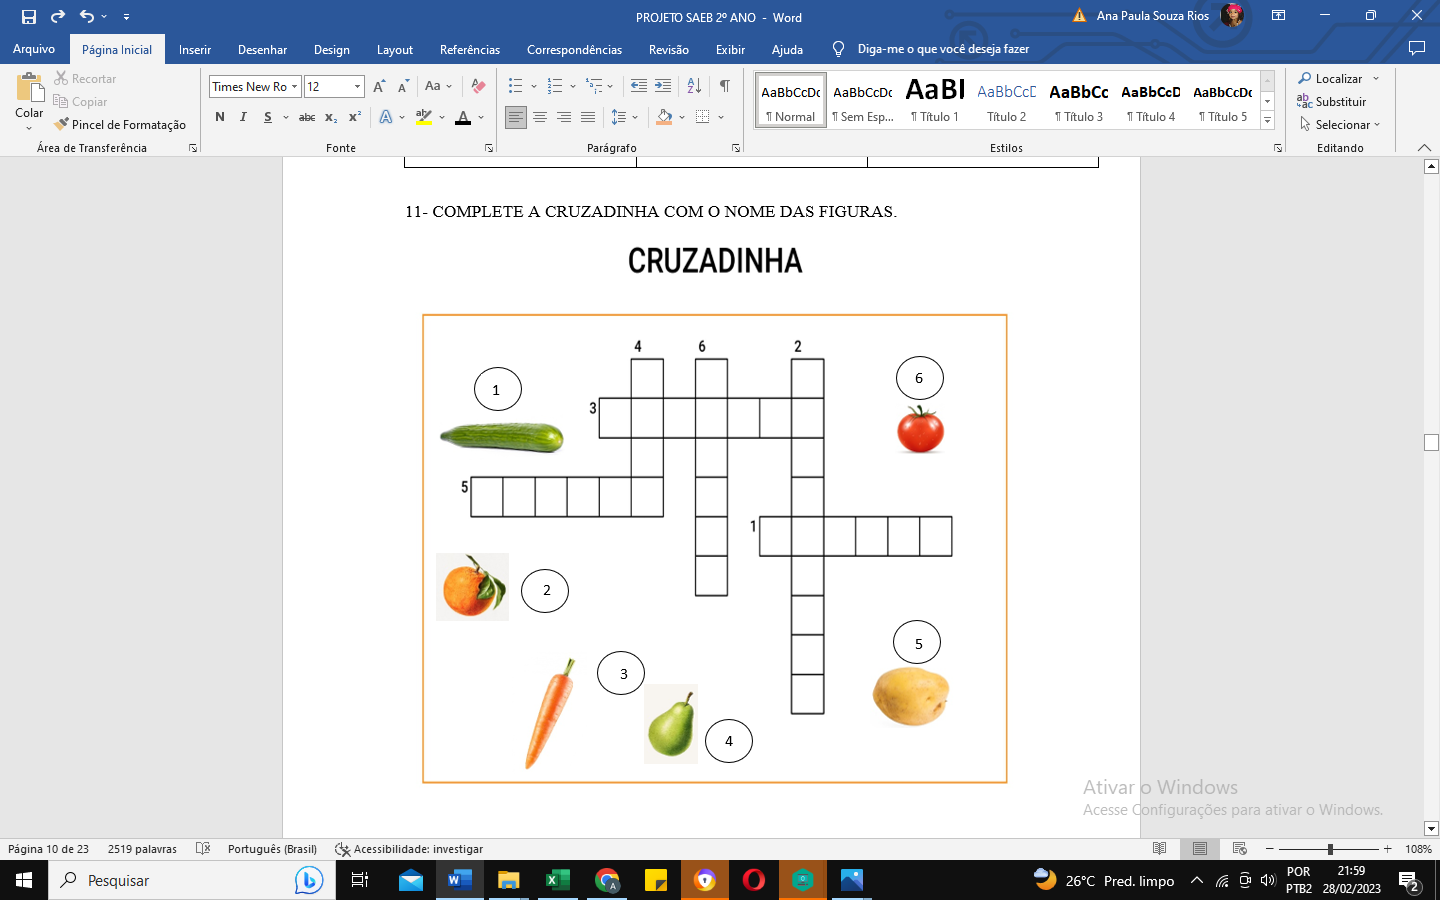
\includegraphics[width=\textwidth]{media/image40.png}
\end{figure}

\num{12} Encontre e pinte as palavras no diagrama.

%\coment{Depois da leitura das palavras, oriente os alunos a localizá-las no diagrama.}

\begin{longtable}[]{@{}llllllll@{}}
\toprule
	TATU -- CABELO -- BONECA -- PANELA -- CAJU\tabularnewline
FADA -- DADO -- VASO -- CAMA -- TAPETE\tabularnewline
\midrule
D & B & F & A & D & A & D & G\tabularnewline
A & C & A & B & E & L & O & U\tabularnewline
G & Y & B & O & C & A & M & A\tabularnewline
S & T & I & N & H & M & A & Q\tabularnewline
P & A & N & E & L & A & D & F\tabularnewline
H & T & O & C & A & J & U & L\tabularnewline
J & U & K & A & D & A & D & O\tabularnewline
T & A & P & E & T & E & Z & X\tabularnewline
K & V & A & S & O & B & G & J\tabularnewline
\end{longtable}

\pagebreak
\colorsec{Treino}

\num{1} Observe o animal que Júlia encontrou enquanto brincava na 
fazenda do Tio Belo.

\begin{figure}[htpb!]
\centering

\includegraphics[width=.9\textwidth]{media/image42.jpeg}
\end{figure}

A palavra que começa com a mesma letra do nome do animal que Júlia encontrou é

\begin{escolha}
\item vaso.

\item gato.

\item bola.

\item foca
\end{escolha}


\num{2} Observe a palavra que Tiago leu para sua professora.

\begin{myquote}
CAJU
\end{myquote}

O nome da figura que termina com a mesma letra da palavra que Tiago leu é

\begin{escolha}
\item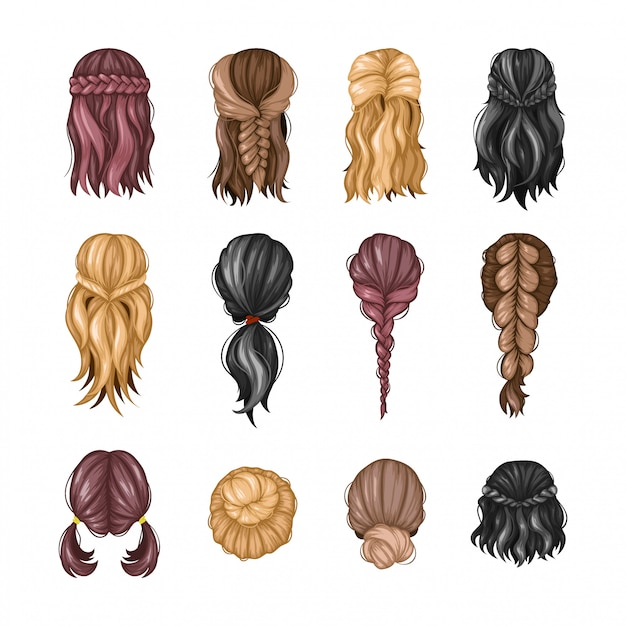
\includegraphics[width=0.79792in,height=0.81667in]{media/image44.jpeg}

\item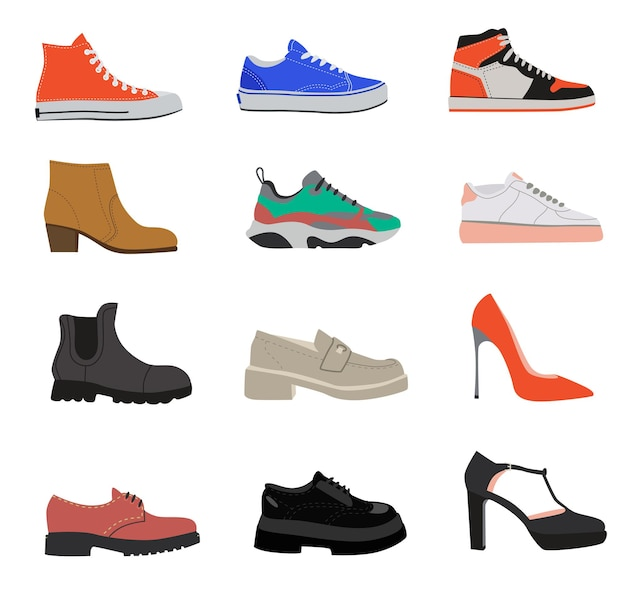
\includegraphics[width=1.02847in,height=0.72292in]{media/image45.jpeg}

\item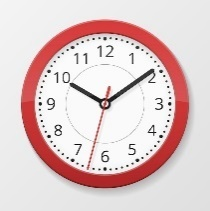
\includegraphics[width=0.79792in,height=0.79931in]{media/image46.jpeg}

\item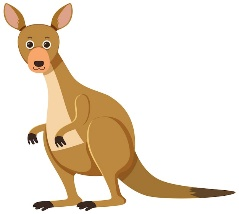
\includegraphics[width=1.08611in,height=0.97222in]{media/image47.jpeg}
\end{escolha}


\num{3} Observe o presente que Bruna ganhou.

\begin{figure}[htpb!]
\centering
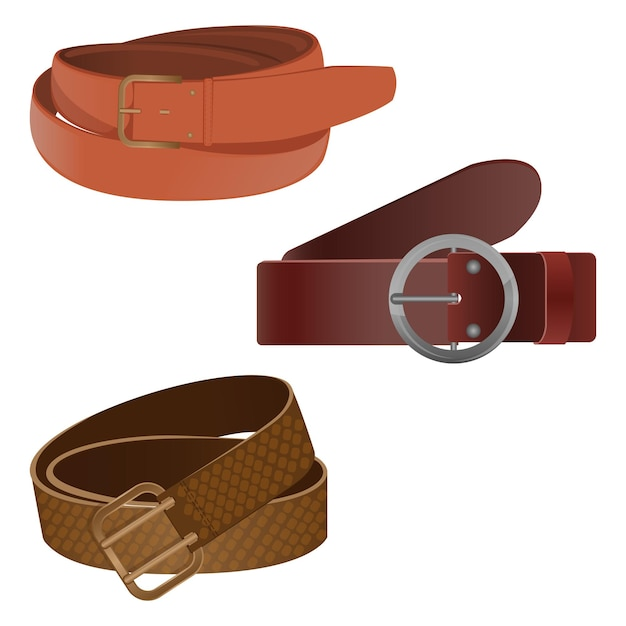
\includegraphics[width=.3\textwidth]{media/image48.jpeg}
\end{figure}

A palavra que começa como o mesmo som da letra do nome do presente de Bruna é

\begin{multicols}{2}
\begin{escolha}
\item cama.

\item cubo.

\item cebola.

\item cocada.
\end{escolha}
\end{multicols}

\chapter{Lendo e escrevendo}
\markboth{Módulo 2}{}

\vspace*{-1.5cm}

\colorsec{Habilidades do SAEB}

\begin{itemize}
\item Ler palavras.
\item Escrever palavras.
\item Ler frases.
\end{itemize}

\colorsec{Habilidades da BNCC}

\begin{itemize}
\item EF02LP04, EF02LP05.
\end{itemize}

\conteudo{Para escrever uma palavra, você precisa usar as letras, que
se dividem em vogais e consoantes.

As vogais são 

\begin{myquote}
\textbf{A -- E -- I -- O -- U} 
\end{myquote}

e as consoantes são

\begin{myquote}
\textbf{B -- C -- D -- F -- G -- H -- J -- K -- L -- M -- N -- P -- Q -- R -- S
-- T -- V -- W -- Y -- X -- Z.}
\end{myquote}

As palavras são lidas e escritas da esquerda para a direita.

\begin{myquote}
$\longrightarrow$

\textbf{GRAVIOLA LÂMPADA AVIÃO LARANJA }
\end{myquote}

Existem diferentes maneiras de compor a sílaba de uma palavra. 

\textbf{CONSOANTE + VOGAL}: é o que acontece nas três sílabas das 
palavras \textit{sapato} e \textit{telefone}: SA-PA-TO e TE-LE-FO-NE

\textbf{VOGAL}: é o que acontece na segunda sílaba das  
palavras \textit{saída} e \textit{saúde}: SA-Í-DA e SA-Ú-DE

\textbf{CONSOANTE + VOGAL + CONSOANTE}: é o que acontece na 
primera sílaba das palavras \textit{porta} e \textit{cortina}:
POR-TA e COR-TI-NA

\textbf{CONSOANTE + CONSOANTE + VOGAL}: é o que acontece na 
primera sílaba da palavra \textit{criança} e na última
sílaba da palavra \textit{livro}: CRI-AN-ÇA e LI-VRO 

Observe o quadro abaixo, com outros exemplos:\bigskip

\noindent{\tiny
\begin{tabular}{l|l|l|l|l|}
\cline{2-5}
 & \textbf{GRAVIOLA} & \textbf{LÂMPADA} & \textbf{AVIÃO} & \textbf{LARANJA} \\ \hline
\multicolumn{1}{|l|}{\textbf{FORMAÇÃO SILÁBICA CV}} & GRA - \textbf{VI} - O - \textbf{LA} & LÂM - \textbf{PA} - \textbf{DA} & A - \textbf{VI} -ÃO & \textbf{LA} - RAN - \textbf{JA} \\ \hline
\multicolumn{1}{|l|}{\textbf{FORMAÇÃO SILÁBICA V}} & GRA - VI - \textbf{O} - LA & \multicolumn{1}{c|}{*} & \textbf{A} - VI -ÃO & \multicolumn{1}{c|}{*} \\ \hline
\multicolumn{1}{|l|}{\textbf{FORMAÇÃO SILÁBICA CVC}} & \multicolumn{1}{c|}{*} & \textbf{LÂM} - PA - DA & \multicolumn{1}{c|}{*} & LA - \textbf{RAN} - JA \\ \hline
\multicolumn{1}{|l|}{\textbf{FORMAÇÃO SILÁBICA CCV}} & \textbf{GRA} - VI - O - LA & \multicolumn{1}{c|}{*} & \multicolumn{1}{c|}{*} & \multicolumn{1}{c|}{*} \\ \hline
\end{tabular}
}


Note que, em todas as formações das sílabas, aparecem vogais. Isso
acontece porque não existe sílaba sem vogal, isto é, uma  sílaba não
se forma só com consoantes.

Observe a frase a seguir:

\begin{myquote}
\textbf{O avião pousou cedo.}
\end{myquote}

Você conhece esse sinal em cima da letra A da palavra \textbf{avião}?

Esse sinal é o \textbf{til}, usado nas vogais A e O para marcar a
nasalidade presente na sílaba.

As marcas de nasalidade aparece também nas letras M e N, no final da
sílaba. É o que acontece, por exemplo, com as seguintes palavras:

\begin{myquote}
\textbf{LÂMPADA E LARANJA}
\end{myquote}

A letra \textbf{M} é utilizada antes das consoantes P e B.  
A letra \textbf{N} é usada antes das demais consoantes, nunca 
no final das palavras.
}

\colorsec{Atividades}

\num{1} Escreva os nomes das figuras.

%\coment{Leve o alfabeto móvel para a sala de aula. Convide as crianças para manusear as letras; em seguida, oriente-as a formar as palavras que nomeiam as figuras. Sugira a elas que, antes de escrever, elas devem pronunciar a palavra, escrevendo-a por sílabas ou pedacinhos.}


\begin{figure}[htpb!]
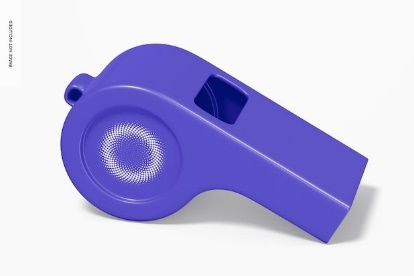
\includegraphics[width=1.46154in,height=0.93603in]{media/image49.jpeg}
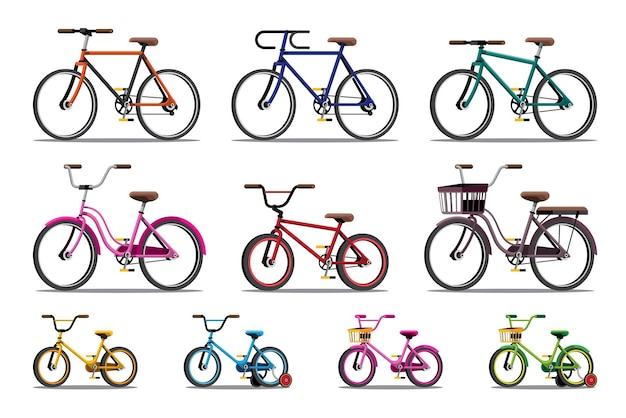
\includegraphics[width=1.16587in,height=0.93269in]{media/image50.jpeg}
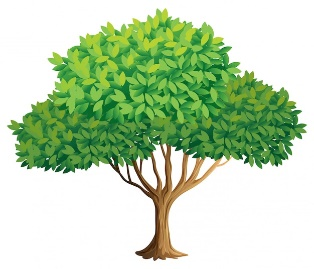
\includegraphics[width=1.42308in,height=1.21950in]{media/image51.jpeg}
\end{figure}

\reduline{Apito\hfill}

\reduline{Bicicleta\hfill}

\reduline{Árvore\hfill}

\begin{figure}[htpb!]
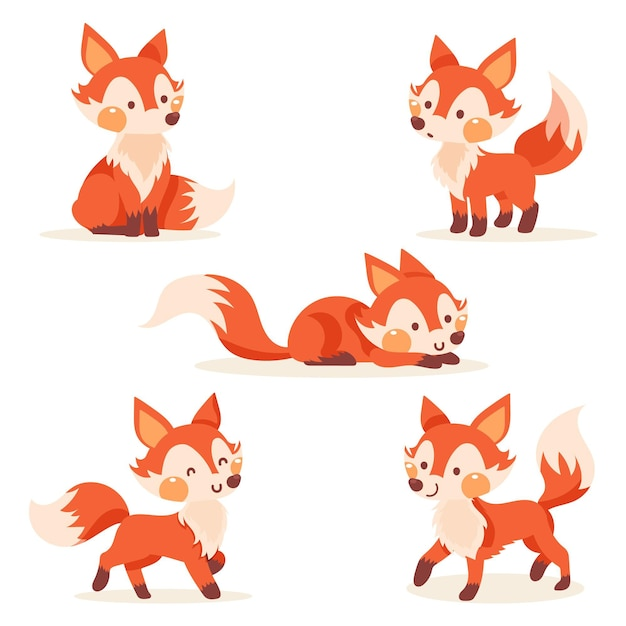
\includegraphics[width=1.10833in,height=1.00903in]{media/image52.jpeg}
\includegraphics[width=0.85556in,height=0.92222in]{media/image53.jpeg}
\includegraphics[width=0.79808in,height=0.79808in]{media/image54.jpeg}
\end{figure}

\reduline{Bola\hfill}

\reduline{Raposa\hfill}

\reduline{Gaiola\hfill}

\begin{figure}[htpb!]
\includegraphics[width=0.91319in,height=1.16319in]{media/image55.jpeg}
\includegraphics[width=1.62569in,height=1.25000in]{media/image56.jpeg}
\includegraphics[width=0.93990in,height=1.27885in]{media/image57.jpeg}
\end{figure}

\reduline{Pera\hfill}

\reduline{Pedra\hfill}

\reduline{Unha\hfill}

\pagebreak
\num{2} Separe as sílabas das palavras, depois circule as sílabas formadas por
consoante + consoante + vogal.

%\coment{Leia as palavras com os alunos, orientando-os a identificar vogais e consoantes. Também é possível montar algumas palavras com o alfabeto móvel. Em seguida, peça a eles que batam palmas cada vez que um pedacinho da palavra for pronunciado.}

\begin{longtable}[]{@{}ll@{}}
\toprule
\textbf{PRATO} & \rosa{Pra - to}\tabularnewline
\midrule
\textbf{FORMIGA} & \rosa{For- mi -ga}\tabularnewline
\midrule
\textbf{BRAÇO} & \rosa{Bra -ço}\tabularnewline
\midrule
\textbf{DRAGÃO} & \rosa{Dra- gão}\tabularnewline
\midrule
\textbf{CRAVO} & \rosa{Cra -- vo}\tabularnewline
\bottomrule
\end{longtable}

\num{3} Ligue as palavras com seu desenho.

%\coment{Leve para sala as palavras dentro de uma sacola. Cada criança deve pegar uma palavra da sacola para fazer a leitura. Depois proponha a atividade.}

Bicicleta \hfill\includegraphics[width=.1\textwidth]{media/image59.png}

Janela \hfill\includegraphics[width=.1\textwidth]{media/image60.png}

Borboleta \hfill\includegraphics[width=.1\textwidth]{media/image61.png}

Dragão \hfill\includegraphics[width=.1\textwidth]{media/image62.png}

Avião \hfill\includegraphics[width=.1\textwidth]{media/image63.png}

Prego \hfill\includegraphics[width=.1\textwidth]{media/image64.jpeg}

Pomba \hfill\includegraphics[width=.1\textwidth]{media/image65.png}

Manga \hfill\includegraphics[width=.1\textwidth]{media/image66.png}


\pagebreak
\num{4} Pinte no diagrama as palavras do quadro abaixo.

%\coment{Faça a leitura das palavras com os alunos aproveite esse momento para trabalhar a função da escrita.}

\begin{quote}\parindent=0em
\vspace*{-.5cm}
\begin{multicols}{3}
PIÃO

CAMA

LEÃO

PEDRA

ABACATE

SAPO

PATO

SABÃO

TRATOR

GRAMA

CISNE
\end{multicols}
\end{quote}

\begin{longtable}[]{@{}llllllllll@{}}
\toprule
P & I & Ã & O & D & O & W & E & I & S\tabularnewline
F & H & P & I & S & A & B & Ã & O & A\tabularnewline
S & J & L & S & J & U & Y & U & J & P\tabularnewline
L & O & A & B & A & C & A & T & E & O\tabularnewline
E & U & I & D & A & S & A & L & K & A\tabularnewline
à & A & B & G & C & A & Y & J & G & P\tabularnewline
O & S & A & P & A & T & O & P & R & E\tabularnewline
Z & D & R & F & D & M & E & C & A & D\tabularnewline
L & T & R & A & T & O & R & Q & M & R\tabularnewline
B & U & G & T & E & Y & E & & A & A\tabularnewline
A & C & I & S & N & E & O & P & U & O\tabularnewline
L & O & L & O & C & A & M & A & A & G\tabularnewline
\bottomrule
\end{longtable}

%\coment{R: pião -- cama -- leão- pedra- abacate- sapo- cama- pato -- sabão -- trator -- grama- cisne.}

\num{5} Coloque o til nas palavras sempre que necessário.

%\coment{Construa com os alunos critérios para identificar as marcas de nasalidade de uma palavra. Sugira que leiam as palavras em voz alta e posicionem os dedos indicador e polegar sobre o nariz ao pronunciar palavras com esses sons, para perceberem a diferença, por exemplo, entre a pronúncia de palavras como \textit{lá} e \textit{lã}, \textit{manha} e \textit{manhã}. Explique que o til acompanha apenas as vogais A e O.}

\begin{multicols}{3}
IRMAO

SALA

MAO

PATO

MAÇA

VILA

MOLA

MANHA

LA
\end{multicols}

\num{6} Observe a marca de nasalização e complete as palavras com M ou N.

%\coment{Siga as orientações da questão anterior, aguçando a atenção das crianças quanto à diferença de pronúncia de palavras como \textit{pote} e \textit{ponte} e \textit{rapa} e \textit{rampa}. Reforce a ideia de M sempre antes de B, e N antes de outras consoantes.}

\begin{multicols}{3}
LÂ\reduline{M}PADA

CA\reduline{M}PO

LARA\reduline{N}JA

TRO\reduline{N}CO

VE\reduline{N}TO

PO\reduline{M}BA

U\reduline{M}BIGO

PO\reduline{N}TE

RA\reduline{M}PA

BO\reduline{M}BOM

TE\reduline{M}PO

PI\reduline{N}TA
\end{multicols}

\num{7} Observe as imagens e escreva uma frase para cada uma.

%\coment{Explore as imagens com as crianças e oriente a construção das frases.}

\begin{figure}[htpb!]
\centering
\includegraphics[width=.5\textwidth]{media/image67.jpeg}
\end{figure}

\reduline{Uma resposta possível é \textit{As crianças andam a cavalo}.\hfill}
\linhas{1}

\begin{figure}[htpb!]
\centering
\includegraphics[width=.5\textwidth]{media/image68.jpeg}
\end{figure}

\reduline{Uma resposta possível é \textit{A menina leva flores no carrinho}.\hfill}
\linhas{1}

\pagebreak
\num{8} Leia as frases a seguir e faça um desenho para representar.

%\coment{Oriente a leitura das frases explorando com as crianças o conteúdo de cada uma delas e as diferentes possibilidades de representação.}

\begin{myquote}
O CAVALO GOSTA DE CORRER.
\end{myquote}

\begin{mdframed}[linewidth=2pt,linecolor=salmao]
\vspace{7cm}
\end{mdframed}

\begin{myquote}
O MENINO JOGA BOLA.
\end{myquote}

\begin{mdframed}[linewidth=2pt,linecolor=salmao]
\vspace{7cm}
\end{mdframed}

\begin{myquote}
O PÁSSARO CANTA FELIZ.
\end{myquote}

\begin{mdframed}[linewidth=2pt,linecolor=salmao]
\vspace{7cm}
\end{mdframed}

\begin{myquote}
A ÁRVORE CAIU.
\end{myquote}

\begin{mdframed}[linewidth=2pt,linecolor=salmao]
\vspace{7cm}
\end{mdframed}

%\coment{Respostas pessoais dos alunos.}

\num{9} Forme palavras de acordo com a numeração, depois forme uma frase.

%\coment{Oriente os alunos a formar as palavras. Em seguida, trabalhe a função social de cada palavra para facilitar a construção das frases.}

\begin{longtable}[]{@{}lllll@{}}
\toprule
\begin{minipage}[b]{0.19\columnwidth}\raggedright\strut
1

BO\strut
\end{minipage} & \begin{minipage}[b]{0.19\columnwidth}\raggedright\strut
2

PI\strut
\end{minipage} & \begin{minipage}[b]{0.19\columnwidth}\raggedright\strut
3

NE\strut
\end{minipage} & \begin{minipage}[b]{0.19\columnwidth}\raggedright\strut
4

CO\strut
\end{minipage} & \begin{minipage}[b]{0.19\columnwidth}\raggedright\strut
5

ÃO\strut
\end{minipage}\tabularnewline
\midrule
\endhead
\begin{minipage}[t]{0.19\columnwidth}\raggedright\strut
6

CAM\strut
\end{minipage} & \begin{minipage}[t]{0.19\columnwidth}\raggedright\strut
7

BRA\strut
\end{minipage} & \begin{minipage}[t]{0.19\columnwidth}\raggedright\strut
8

CIS\strut
\end{minipage} & \begin{minipage}[t]{0.19\columnwidth}\raggedright\strut
9

CA\strut
\end{minipage} & \begin{minipage}[t]{0.19\columnwidth}\raggedright\strut
10

ÇO\strut
\end{minipage}\tabularnewline
\midrule
\begin{minipage}[t]{0.19\columnwidth}\raggedright\strut
11

MA\strut
\end{minipage} & \begin{minipage}[t]{0.19\columnwidth}\raggedright\strut
12

JA\strut
\end{minipage} & \begin{minipage}[t]{0.19\columnwidth}\raggedright\strut
13

LA\strut
\end{minipage} & \begin{minipage}[t]{0.19\columnwidth}\raggedright\strut
14

CA\strut
\end{minipage} & \begin{minipage}[t]{0.19\columnwidth}\raggedright\strut
15

PO\strut
\end{minipage}\tabularnewline
\bottomrule
\end{longtable}

\textbf{PALAVRA FRASE}

\begin{itemize}
\item 1 + 3 + 14 \reduline{boneca\mbox{ }\hfill}

\item 7 + 10 \reduline{\mbox{ }\hfill}

\item 2 + 5 \reduline{\mbox{ }\hfill}

\item 6 + 15 \reduline{\mbox{ }\hfill}

\item 8 + 3 \reduline{\mbox{ }\hfill}

\item 12 + 3 + 13 \reduline{\mbox{ }\hfill}

\item 11 + 9 + 4 \reduline{\mbox{ }\hfill}
\end{itemize}

\num{10} Complete os nomes das frutas com as vogais corretas.

%\coment{Reapresente as vogais aos alunos de acordo com as palavras do exercício. Forme as palavras ressaltado sempre que não existe sílaba sem vogal.}

\begin{figure}[htpb!]
\includegraphics[width=.24\textwidth]{media/image69.jpeg}
\includegraphics[width=.24\textwidth]{media/image70.jpeg}
\includegraphics[width=.24\textwidth]{media/image71.jpeg}
\includegraphics[width=.24\textwidth]{media/image72.jpeg}
\end{figure}

\reduline{U}V\reduline{A} \hspace{1.5cm} L\reduline{A}R\reduline{A}NJ\reduline{A} \hspace{1cm} \reduline{A}B\reduline{A}C\reduline{A}X\reduline{I} \hspace{1cm} B\reduline{A}N\reduline{A}N\reduline{A}

\begin{figure}[htpb!]
\includegraphics[width=.24\textwidth]{media/image73.jpeg}
\includegraphics[width=.24\textwidth]{media/image74.jpeg}
\includegraphics[width=.24\textwidth]{media/image75.jpeg}
\includegraphics[width=.24\textwidth]{media/image76.jpeg}
\end{figure}

P\reduline{Ê}R\reduline{A} \hspace{1cm} M\reduline{O}R\reduline{A}NG\reduline{O} \hspace{1cm} G\reduline{O}\reduline{I}\reduline{A}B\reduline{A} \hspace{1cm} M\reduline{A}Ç\reduline{Ã}

\num{11} Organize as palavras de acordo com sua formação silábica.

%\coment{Leve o alfabeto para sala. Explore as vogais e as consoantes com os alunos. Realize com eles a formação de algumas palavras, identificado as diferentes formações silábicas. Brincar de \textbf{forca} é uma boa opção para desenvolver essa atividade.}

\begin{myquote}
ABACAXI -- TRATOR - GRAVIOLA - PRATO -- CAMPO - CISNE - BAÚ
\end{myquote}

{\small
\begin{tabular}{|l|l|l|l|}
\hline
\textbf{\begin{tabular}[c]{@{}l@{}}PALAVRAS COM\\ FORMAÇÃO CV\end{tabular}} & \textbf{\begin{tabular}[c]{@{}l@{}}PALAVRAS COM\\ FORMAÇÃO V\end{tabular}} & \textbf{\begin{tabular}[c]{@{}l@{}}PALAVRAS COM\\ FORMAÇÃO CCV\end{tabular}} & \textbf{\begin{tabular}[c]{@{}l@{}}PALAVRAS COM\\ FORMAÇÃO CVC\end{tabular}} \\ \hline
\rosa{ABACAXI} & \rosa{GRAVIOLA} & \rosa{TRATOR} & \rosa{CISNE} \\ \hline
\rosa{GRAVIOLA} & \rosa{ABACAXI} & \rosa{GRAVIOLA} & \rosa{CAMPO} \\ \hline
\rosa{PRATO} & \rosa{BAÚ} & \rosa{PRATO} &  \\ \hline
\rosa{CAMPO} &  &  &  \\ \hline
\rosa{CISNE} &  &  &  \\ \hline
\rosa{BAÚ} &  &  &  \\ \hline
\end{tabular}
}

\pagebreak
\colorsec{Treino}

\num{1} Mila foi à feira e comprou seu brinquedo preferido com as
econonias de seu cofrinho.

\begin{figure}[htpb!]
\centering
\includegraphics[width=.5\textwidth]{media/image77.jpeg}
\end{figure}

Qual palavra tem a primeira sílaba com a mesma formação da primeira
sílaba do nome do brinquedo de Mila?

\begin{multicols}{2}
\begin{escolha}
\item abacate.

\item janela.

\item traça.

\item prego.
\end{escolha}
\end{multicols}

\num{2} Leia a frase.

\begin{myquote}
\textbf{A menina brinca com bolhas de sabão.}
\end{myquote}

A imagem que representa o que está escrito na frase é

\begin{multicols}{2}
\begin{escolha}
\item\includegraphics[width=0.75159in,height=1.04531in]{media/image78.jpeg}

\item\includegraphics[width=1.23681in,height=1.10139in]{media/image79.jpeg}

\item\includegraphics[width=0.97361in,height=1.05069in]{media/image80.jpeg}

\item\includegraphics[width=0.75437in,height=1.04404in]{media/image81.jpeg}
\end{escolha}
\end{multicols}


\num{3} Veja a palavra nova que Ana aprendeu a ler.

\begin{myquote}
FORMIGA
\end{myquote}

A primeira sílaba da palavra acima tem a mesma formação que a 
primeira sílaba de

\begin{escolha}
\item borboleta.

\item dragão.

\item laranja.

\item garota.
\end{escolha}


\chapter[Encontrando informações no texto]{\Large Encontrando informações no texto}
\markboth{Módulo 3}{}

%Para iniciar este módulo, é possível comentar os tipos dos textos que serão lidos e explorar bastante a oralidade, fazendo diversos questionamentos de informações que estão nos textos.

\colorsec{Habilidade do SAEB}

\begin{itemize}
	\item Localizar informações explícitas em textos
\end{itemize}

\colorsec{Habilidades da BNCC}

\begin{itemize}
\item EF15LP03
\end{itemize}

\conteudo{

\begin{verse}
\textbf{Meu galinho}

Há três noites que eu não durmo\\
Ó lá lá\\
Pois perdi o meu galinho\\
O lá lá\\
Coitadinho o lá lá,\\
Pobrezinho o lá lá\\
Se perdeu lá no jardim.

Ele é branco e amarelo\\
O lá lá\\
Tem a crista vermelhinha\\
O lá lá\\
Bate as asas, o lá lá,\\
Abre o bico o lá lá\\
E faz qui qui ri qui qui
\end{verse}

\fonte{Disponível em: http://www.dominiopublico.gov.br/download/texto/me000588.pdf. Acesso em: 19 abr. 2023. }

Por que ele não dorme?

Onde o galo se perdeu?

Quais são as cores do galo?

Para responder a essas e outras perguntas, você precisa buscar as
informações no texto. Elas estão todas lá, de forma bem clara. 
Basta observar com atenção.

Observe o seguinte cartaz:\bigskip

\noindent\includegraphics[width=\textwidth]{media/image82.png}\bigskip

Está bem claro que esse cartaz contém um pedido de doação de brinquedos.
}

\colorsec{Atividades}

\num{1} Vamos cantar.

%\coment{Convide as crianças para brincar com a música, usando o nome dos alunos da turma. Em seguida faça questionamentos sobre a música: onde a canoa virou? Maria estava sozinha? Alguém socorreu Maria?}

\begin{quote}
\begin{verse}
\textbf{A canoa virou}

A canoa virou,\\
pois deixaram virar.\\
Foi por causa da maria,\\
que não soube remar.

Se eu fosse um peixinho\\
e soubesse nadar,\\
eu tirava a maria\\
do fundo do mar.
\end{verse}

\fonte{Política Nacional de Alfabetização. Cantigas. Disponível em: https://tinyurl.com/yckw7p6b. Acesso em: 19 abr. 2023. }
\end{quote}

\begin{escolha}
\item Escreva o título da música.

\reduline{A canoa virou.\hfill}
\linhas{1}

\item Por que a canoa virou?

\reduline{Maria não soube remar.\hfill}
\linhas{1}

\item Se eu fosse um peixinho o que eu faria?

\reduline{Se eu fosse um peixinho, eu tirava Maria do fundo do mar.\hfill}
\linhas{1}
\end{escolha}

\num{2} Vamos brincar de trem?

%\coment{Convide os alunos para formar um trem. Nesse momento, podem ser trabalhadas as noções de \textbf{lateralidade}: frente, trás, entre. Faça os questionamentos orais para trabalhar a fala e a escuta com as crianças.}

\begin{quote}
\begin{verse}
\textbf{O trem maluco}

O trem maluco,\\
quando sai de Pernambuco,\\
vai fazendo xique-xique\\
até chegar ao Ceará.
\end{verse}
\end{quote}

\begin{escolha}
\item  Encontre e circule o título da música.

\item De onde o trem sai?

\reduline{O trem sai de Pernambuco.\hfill}

\item Para onde o trem vai?

\reduline{O trem vai para o Ceará.\hfill}
\end{escolha}

\num{3} Vamos ler a letra da canção.\enlargethispage{2\baselineskip}

%\coment{Inicialmente, faça a leitura da letra da canção. Em seguida, convide as crianças a cantar. Depois, faça perguntas sobre o conteúdo da letra para trabalhar a oralidade.}

\begin{quote}
\begin{verse}
\textbf{Borboletinha}

Borboletinha\\
está na cozinha\\
fazendo chocolate\\
para a madrinha\\
poti,poti\\
perna de pau\\
olho de vidro\\
e nariz de pica-pau\\
tchau, tchau
\end{verse}

\fonte{Secretaria de Educação da Prefeitura de Diadema. Borboletinha. Disponível em: https://tinyurl.com/3n5ym7w5. Acesso em: 19 abr. 2023. }
\end{quote}

\begin{escolha}
\item Encontre e pinte de azul o nome da música.

\item Onde a borboletinha está?

\reduline{A borboletinha está na cozinha.\hfill}

\item O que ela está fazendo?

\reduline{A borboletinha está fazendo chocolate.\hfill}

\item Para quem é o cochocolate que ela está fazendo?

\reduline{A borboletinha está fazendo chocolate para a madrinha.\hfill}
\end{escolha}

\num{4} Observe esse cartaz.

%\coment{Pergunte as crianças o que elas vem no cartaz. Questione se já participaram de alguma campanha ou se já doaram roupas para outras pessoas. Aproveite e fale da importância de ser solidário.}

\begin{figure}[htpb!]
\centering
\includegraphics[width=.5\textwidth]{media/image83.jpeg}
\end{figure}
%\textbf{\url{http://www.saosebastiao.sp.gov.br/noticia.asp?id=N1122020143810.Acesso} 02 mar. 2023}

\begin{escolha}
\item Qual é a campanha mostrada no cartaz?

\reduline{O cartaz apresenta uma campanha de arrecadação de roupas.\hfill}

\item As roupas devem ser doadas a crianças de que idade?

\reduline{As roupas devem ser doadas a crianças de zero a 3 anos.\hfill}
\end{escolha}

\num{5} Vamos ler com atenção.

%\coment{Leia a receita para as crianças. Depois, pergunte a elas se conhecem esse tipo de texto. Identifique com elas as instruções apresentadas. A seguir, explore o conteúdo da receita, perguntando aos alunos, por exemplo, se conhecem os ingredientes e gostam deles.}

%Paulo: acredito que seria interessante colocar a receita abaixo em um box que lembrasse uma folha de papel, pautada ou não, se possível com uma fonte que lembre letra cursiva. 
\begin{quote}
\textbf{Macarrão de panela de pressão}

\textbf{Ingredientes}

%\includegraphics[width=1.94097in,height=1.14722in]{media/image84.jpeg}1

\begin{itemize}
\item 1 pacote de macarrão tipo parafuso

\item 1 saquinho molho de tomate

\item 1 caixa de creme de leite

\item Sal a gosto

\item Alho e cebola a gosto

\item 2 medidas do recipiente do molho de tomate de água

\end{itemize}

\textbf{Modo de fazer}

Em uma panela de pressão, frite o alho e a cebola. Depois, jogue o
macarrão e o molho de tomate e misture tudo. Aproveite o recipiente
do molho de tomate (o saquinho ou o pote): encha-o com água duas vezes
e jogue-a na panela.

Depois feche a panela e coloque no fogo. Assim que a panela pegar a
pressão, desligue, mas não abra e nem tire o pino: espere sair toda 
a pressão sozinha, lentamente. Quando isso acontecer, abra, mexa o
macarrão e coloque a caixa de creme de leite. Tempere com o sal a gosto.
Pronto! É só comer. 
\end{quote}

%Felipe ou Fábia: alterei esta receita (mandei mensagem no Odoo). Por isso, o link a seguir não é mais necessário: http://educacao.diadema.sp.gov.br/educacao/attachments/article/749/atividade\%209\%20semana\%20fase\%20I\%20Drummond.pdf.Acesso} 02 mar. 2023.
%https://www.freepik.com/premium-photo/spaghetti-dish-white-background\_4396472.htm\#query=MACARR\%C3\%83O\&position=8\&from\_view=search\&track=sph

\begin{escolha}
\item Qual é o nome do prato explicado na receita?

\reduline{O nome do prato explicado na receita é macarrão de panela de pressão.\hfill}

\item Encontre no texto e pinte de verde o nome do utensílio usado para
conzinhar o macarrão.

\reduline{O aluno deve pintar de verde a expressão ``panela de pressão''.\hfill}

\pagebreak
\item Agora escreva o nome de três ingredientes usados para fazer a receita.

\reduline{Os ingredientes usados para fazer a receita são macarrão, molho, creme de leite, sal, alho, cebola e água. O aluno deve escolher três deles.\hfill}
\end{escolha}

\num{6} Vamos cantar.

\begin{quote}
\begin{verse}
\textbf{Meu chapéu}

O meu chapéu tem três pontas,\\
tem três pontas o meu chapéu.\\
Se não tivesse três pontas,\\
não seria o meu chapéu.
\end{verse}

\fonte{Secretaria de Educação da Prefeitura de Diadema. Borboletinha. Disponível em: http://educacao.diadema.sp.gov.br/educacao/attachments/article/749/atividade\%209\%20semana\%20fase\%20I\%20Drummond.pdf. Acesso em: 19 abr. 2023. }
\end{quote}

\begin{escolha}
\item Quantas pontas tem o chapéu que aparece na canção?

\reduline{O chapéu descrito na letra da canção tem três pontas.\hfill}

\item Como você imagina que é esse chapéu? Desenhe.

\begin{mdframed}[linewidth=2pt,linecolor=salmao,roundcorner=10pt]
\coment{Resposta pessoal.}
\vspace{4cm}
\end{mdframed}
\end{escolha}

\num{7} Leia as informações do cartaz.

%\coment{Explore as informações do cartaz: a campanha de vacinação, o período em que acontece e a faixa etária a que se destina. Pergunte aos alunos se eles entendem o que significa a gotinha branca e peça-lhes que expliquem.}

\begin{figure}[htpb!]
\centering
\includegraphics[width=.5\textwidth]{media/image85.jpeg}
\end{figure}

%\url{https://barreiras.ba.gov.br/segunda-etapa-da-campanha-de-vacinacao-contra-o-sarampo-comeca-na-quinta-feira-14-em-barreiras/} Acesso 02 mar. 2023.

\begin{escolha}
\item Qual é a campanha divulgada no cartaz?

\reduline{A campanha divulgada no cartaz é a de vacinação contra o sarampo.\hfill}

\item Para quem é indicada essa vacinação?

\reduline{A vacinação é indicada para jovens e adultos de 20 a 29 anos.\hfill}

\item Em que período vai acontecer a campanha?
	
\reduline{A campanha vai acontecer de 18 a 30 de Novembro.\hfill}
\end{escolha}

\num{8} Leia o texto.

%\coment{Depois de cantar a canção e ler a letra, é interessante fazer uma dobradura do chapéu.}

\begin{quote}
\begin{verse}
\textbf{Marcha soldado}

Marcha soldado,\\
cabeça de papel.\\
Se não marchar direito,\\
vai preso pro quartel.

O quartel pegou fogo,\\
a polícia deu sinal.\\
Acode, acode, acode,\\
a bandeira nacional.
\end{verse}

\fonte{Política Nacional de Alfabetização. Cantigas. Disponível em: https://alfabetizacao.mec.gov.br/images/conta-pra-mim/livros/versao\_digital/cantigas\_versao\_digital.pdf. Acesso em: 19 abr. 2023. }
\end{quote}

\begin{escolha}
\item Localize no texto e pinte de vermelho como é a cabeça do soldado.

\item O que acontece com o soldado se não marchar direto?

\reduline{Se não marchar direito, o soldado vai preso.\hfill}

\end{escolha}

\num{9} Vamos cantar.

\begin{quote}
\begin{verse}
\textbf{Dona aranha}

A Dona Aranha subiu pela parede\\
veio a chuva forte e a derrubou\\
já passou a chuva\\
o sol já vai surgindo\\
e a Dona Aranha continua a subir
\end{verse}

\fonte{https://www2.bauru.sp.gov.br/arquivos/arquivos\_site/sec\_educacao/atividades\_pedagogica\_distancia/1;Infantil/49;EMEI\%20Maria\%20Elizabet\%20Camilo\%20de\%20P\%C3\%A1dua/5;PROF.\%C2\%AA\%20REBECA/Atividades\%20de\%2012\%20a\%2016\%20de\%20abril\_Infantil\%20II\%20B\_Prof\%C2\%AA\%20Rebeca.pdf.
Acesso 11 mar. 2023.}
\end{quote}

\begin{escolha}
\item Escreva o nome do animal que aparece na música.

\reduline{Aranha\hfill}

\pagebreak
\item Quem derrubou a Dona Aranha?

\reduline{A Dona Aranha foi derrubada pela chuva forte.\hfill}

\end{escolha}

\num{10} Vamos cantar.

\begin{quote}
\begin{verse}
\textbf{Pai Francisco}

Pai Francisco entrou na roda\\
tocando seu violão\\
vem de lá Seu Delegado\\
e Pai Francisco foi pra prisão.
\end{verse}
\end{quote}

%Tentei de todas as formas acessar a página a seguir, mas não consegui de jeito nenhum. Deve ser conteúdo restrito {http://servicos.rolandia.pr.gov.br/educacao/wp-content/uploads/aulas_online/cmeis/JOSEMARIA\%20ESCRIV\%C3\%81/INFANTIL-1/2021/16\%C2\%BAROT-I1B.pdf}Acesso 11 mar. 2023.

\begin{escolha}
\item Qual é o nome da canção?

\reduline{O nome da canção é ``Pai Francisco''.\hfill}

\item Desenhe o instrumento musical que Pai Francisco estava tocando.

\begin{mdframed}[linewidth=2pt,linecolor=salmao,roundcorner=10pt]
\vspace{8cm}
\end{mdframed}
\end{escolha}

\colorsec{Treino}

\num{1}

\begin{quote}
\begin{verse}
\textbf{Pintinho}

Meu pintinho amarelinho\\
cata aqui na minha mão,\\ 
na minha mão.\\
Quando quer comer bichinho,\\ 
com seu pezinho\\ 
ele cisca o chão.

Ele bate as asas,\\
ele faz piu-piu,\\ 
mas tem muito medo do gavião.
\end{verse}

\fonte{Domínio Público. Pintinho. Disponível em:
http://www.dominiopublico.gov.br/download/texto/me000588.pdf.
Acesso em: 19 abr. 2023.}
\end{quote}

O que o pintinho faz quando quer comer bichinho?

\begin{escolha}
	\item Cisca o chão.

	\item Bate as asas.

	\item Cata na mão.

	\item Faz piu-piu.
\end{escolha}

\pagebreak
\num{2} Leia o texto a seguir.

\begin{quote}
\begin{verse}
\textbf{Pombinha branca}

Pombinha branca \\
O que está fazendo?\\
Lavando a roupa\\
Do casamento.

A roupa é suja\\
É cor-de-rosa\\
Pombinha branca\\
É preguiçosa.

\end{verse}

\fonte{Domínio Público. Pombinha branca. Disponível em: http://www.dominiopublico.gov.br/download/texto/me000588.pdf. Acesso em: 19 abr. 2023.  }
\end{quote}

A pombinha é considerada preguiçosa porque

\begin{escolha}
	\item vai casar.

	\item a roupa está suja.

	\item só tem roupas cor-de-rosa.

	\item porque está lavando roupa.
\end{escolha}

\pagebreak
\num{3} Leia o texto.

\begin{quote}
\begin{verse}
\textbf{O tubo de cola}

O tubo de cola saiu da gaveta\\
caiu no tapete da sala.\\
a bola pulou no tapete melado e ficou colada na cola.\\
aí, a bola falou:\\
--- sapato, me ajuda!\\
o sapato ajudou.\\
deu um peteleco na bola\\
a bola melada colou no sapato.
\end{verse}

%Aqui temos um problema: o texto usado não está em área aberta do site. Não me preocupei com a diagramação do texto acima e da questão em geral.  

\fonte{https://portal.educacao.go.gov.br/wp-content/uploads/2021/04/Atividade-7-2o-ano-LP-LOCALIZAR-INFORMACOES-EXPLICITAS-EM-TEXTOS-E-EM-IMAGENS-GENERO-CONTOS.pd}
\end{quote}

De onde saiu o tubo da cola?

\begin{escolha}
\item DA BOLA

\item DO TAPETE.

\item DO SAPATO.

\item DA GAVETA.
\end{escolha}

\chapter{Para que serve este texto?}
\markboth{Módulo 4}{}

%Para iniciar o módulo, apresente os textos aos alunos pergunte se eles conhecem algum deles. Em seguida, explique a função de cada texto e a quem ele se destina.

\colorsec{Habilidade do SAEB}

\begin{itemize}
\item Reconhecer a finalidade de um texto.
\end{itemize}

\colorsec{Habilidade da BNCC}

\begin{itemize}
\item EF15LP01.
\end{itemize}

\conteudo{Você sabe para que servem os textos?

Existem vários tipos de textos, com linguagem e estrutura próprias e com 
diferentes funções.

Veja alguns deles e suas funções.

\includegraphics[width=.5\textwidth]{media/image86.jpeg}
\includegraphics[width=.5\textwidth]{media/image87.png}

\includegraphics[width=.5\textwidth]{media/image90.jpeg}
\includegraphics[width=.5\textwidth]{media/image92.png}
%\includegraphics[width=1.97452in,height=2.09063in]{media/image91.png}
}

%\textbf{https://www.flickr.com/photos/cbnsp/8264557482/in/photostream/}
%\textbf{https://agenciadenoticias.uniceub.br/sem-categoria/df-supera-80-mil-casos-suspeitos-de-dengue-e-ja-e-mais-que-o-triplo-do-total-do-ano-de-2021/}
%\textbf{https://www.freepik.com/free-photo/calendar-agenda-event-meeting-reminder-schedule-graphic-concept\_17132741.htm\#query=AGENDA\&position=30\&from\_view=search\&track=sph}

\colorsec{Atividades}

\num{1} Bel vai à padaria e quer deixar um aviso para sua tia. 
Marque com um X o texto que ela deve usar.

%\coment{Pergunte aos alunos se eles conhecem esses textos e explique a função de cada um deles.}

\includegraphics[width=.3\textwidth]{media/image93.jpeg}
\includegraphics[width=.3\textwidth]{media/image94.jpeg}
\includegraphics[width=.3\textwidth]{media/image97.png}

%\textbf{https://www.guarapari.es.gov.br/noticia/ler/285/setac-realiza-campanha-de-arrecadacao-de-roupas}

%\textbf{ttps://pt.wikipedia.org/wiki/Agenda\#/media/Ficheiro:Agenda.jpg}

\pagebreak

\num{2} Tamires vai convidar sua prima para a sua festa de formatura. 
Enconte e circule com lápis verde o texto que ela vai usar. 

%\coment{Retome as orientações anteriores para realizar a atividade.}

\includegraphics[width=.5\textwidth]{media/image100.png}
\includegraphics[width=.5\textwidth]{media/image103.png}

%\textbf{https://saltinho.sp.gov.br/paginas/portal/noticia?id=591}

\num{3} Pinte o quadrinho do texto que serve para informar o leitor.

%\coment{Explique a função de cada texto para a turma. Além disso, leve os nomes dos textos em uma caixinha e peça às crianças que sorteiem um deles. Depois, promova uma discussão sobre o texto sorteado.}

\begin{boxlist}
\boxitem{\white{X}} Convite

\boxitem{\white{X}} Notícia

\boxitem{\white{X}} Agenda 

\boxitem{\white{X}} Receita

\boxitem{\white{X}} Cartaz 

\boxitem{\white{X}} Tirinha
\end{boxlist}

\pagebreak
\num{4} No caça-palavras, existem sete nomes de tipos de textos. 
Encontre e pinte cada um deles.  

\begin{myquote}
\begin{multicols}{2}
AGENDA

NOTÍCIA

RECEITA

CONVITE

LISTA

VERBETE

TIRINHA
\end{multicols}
\end{myquote}

%\coment{Poderá usar a sugestão anterior para realizar a atividade.}

\begin{figure}[htpb!]
\includegraphics[width=\textwidth]{media/image104.jpeg}
\end{figure}

%\coment{Resposta: \includegraphics[width=2.42537in,height=2.09849in]{media/image105.jpeg}}

\pagebreak
\num{5} Observe esse texto.

%\coment{Leia o texto junto com as crianças. Em seguida, pergunte a elas se conhecem os ingredientes e se sabem como a receita deve ser seguida. Explique a função das receitas e onde geralmente elas são encontradas.}

\begin{figure}[htpb!]
\includegraphics[width=\textwidth]{media/image106.jpeg}
\end{figure}

%\textbf{https://www.flickr.com/photos/cbnsp/8263487889/in/photostream/ Acesso 03 mar. 2023.}

\begin{escolha}
\item Qual é o nome desse texto?

\reduline{O nome desse texto é ``receita''.\hfill}

\item Para que serve esse texto?

\reduline{A receita serve para ensinar a fazer comida.\hfill}

\item Escreva dois nomes de ingredientes da receita.

\reduline{Os ingredientes são iogurte, hortelã picada, suco de limão, azeite sal.\hfill}
\end{escolha}

\pagebreak
\num{6} Veja esse texto.

%\coment{Explore as informações do cartaz, fazendo, por exemplo, as seguintes perguntas: para que ele serve? A qual grupo é destinado? Quem o produziu?}

\begin{figure}[htpb!]
\includegraphics[width=\textwidth]{media/image107.jpeg}
\end{figure}

%\fonte{https://www.valparaiso.sp.gov.br/portal/noticias/0/3/794/valparaiso-realiza-campanha-de-vacinacao-contra-paralisia-infantil-e-sarampo. Acesso 03 mar. 2023.}

\begin{escolha}
\item Como é chamado esse texto?

\reduline{Esse texto é chamado de cartaz.\hfill}

\item Para que ele serve?

\reduline{Esse texto serve para informar sobre a vacinas.\hfill}

\item Para qual grupo ele é destinando?

\reduline{Esse texto é destinado às crianças.\hfill}
\end{escolha}

\pagebreak
\num{7} Tati gosta de contar história para divertir seus amigos.
Marque com um X o texto que ela deve usar.

\includegraphics[width=.5\textwidth]{media/image110.png}
\includegraphics[width=.5\textwidth]{media/image109.png}

\includegraphics[width=.5\textwidth]{media/image108.jpeg}

%\url{https://agenciadenoticias.uniceub.br/sem-categoria/df-supera-80-mil-casos-suspeitos-de-dengue-e-ja-e-mais-que-o-triplo-do-total-do-ano-de-2021/}
%https://lizeseusamigos.org.br/tirinhas/tirinhas-tres

\num{8} Produza um texto para organizar os itens de uma compra.

%\coment{Pergunte aos alunos se eles conhecem esse tipo de texto. Dialogue com eles sobre a função e estrutura de listas de compras.}

\begin{itemize}
\item \reduline{Resposta pessoal\hfill}

\item \reduline{\mbox{}\hfill}

\item \reduline{\mbox{}\hfill}

\item \reduline{\mbox{}\hfill}

\item \reduline{\mbox{}\hfill}

\item \reduline{\mbox{}\hfill}

\item \reduline{\mbox{}\hfill}
\end{itemize}

\pagebreak
\num{9} Fernanda tem uma reunião no dia 03 de março de 2023. Onde ela
deve anotar esse compromisso?

\reduline{Fernanda deve anotar o compromisso na agenda.\hfill}

\num{10} No dia do aniversário de Samanta, sua madrinha fez um bolo de
chocolate. Pinte o balão com o texto que ela usou para preparar o bolo.

\begin{comment}
\begin{figure}[htpb!]
\includegraphics[width=\textwidth]{media/confederado.png}
\end{figure}
\end{comment}

\pagebreak
\colorsec{Treino}

\num{1} Observe o texto que ana recebeu de sua prima.

\begin{comment}
\begin{figure}[htpb!]
\includegraphics[width=.5\textwidth]{media/confederado2.png}
\end{figure}
\end{comment}

%\textbf{\url{https://www.flickr.com/photos/cbnsp/8263487889/in/photostream/} Acesso 03 mar. 2023.}

Esse texto serve para

\begin{escolha}
	\item Ensinar.

	\item Informar.

	\item Convidar.

	\item Anunciar.
\end{escolha}

\pagebreak
\num{2} Observe o cartaz que Mariana colou no mural da farmácia.

\begin{figure}[htpb!]
\centering
\includegraphics[width=.6\textwidth]{media/image115.png}
\end{figure}

Esse cartaz é destinado aos donos de 

\begin{escolha}
	\item Gatos e cavalos.

	\item Cachorros e ovelhas.

	\item Cavalos e cachorros.

	\item Cachorros e gatos.
\end{escolha}

\num{3} João quer apresentar as características do seu animal selvagem
preferido para seus amigos.

O texto que ele vai usar é

\begin{escolha}
	\item Receita.

	\item Bilhete.

	\item Verbete.

	\item Notícia.
\end{escolha}

\chapter{Encontrando o assunto do texto}
\markboth{Módulo 5}{}

\vspace*{-1cm}
\enlargethispage{2\baselineskip}

\colorsec{Habilidade do SAEB}

\begin{itemize}
\item Inferir o assunto de um texto verbal.
\end{itemize}

%\coment{Para realizar as atividades desse módulo, é necessário ler junto com os alunos todos os textos, explorando a tipologia, título, personagens, e informações nele contidas, levantado hipóteses sobre do assunto dos diferentes textos.}

\conteudo{Para entender o assunto de um texto, você pode levantar
hipóteses, analisar, comparar, estabelecer relações a partir das
afirmações e das partes nele contidas.

Vamos ler o texto a seguir com atenção.

\begin{quote}
\textbf{A galinha e a pérola}

Uma galinha estava esfomeada, por isso começou a zanzar atrás do
galinheiro. Havia ali uma pequena lixeira dos humanos, que sempre
acabavam deixando cair algumas migalhinhas de pão ou pedacinhos de 
bolo saborosos, que a galinha petiscava com muito gosto. No meio
desses restos, a galinha mastigou uma pedra dura, mas muito preciosa:
``uma pérola!'', ela exclamou ``essa pedrinha 
brilhante vale muito para os humanos, mas não significa nada para
mim, que  preferia ter encontrado um grãozinho de milho para encher
a pança \ldots''. E continuou saboreando os restinhos. 

\textbf{Moral da história}: nem todo mundo dá valor para as mesmas
coisas. 
\end{quote}

O texto acima é chamado de \textbf{fábula}. Nele, um animal age
como ser humano. A \textbf{moral da história} orienta o leitor a
entender o assunto do texto. No caso da fábula acima, a pérola é
preciosa para os humanos, mas não tem importância para a galinha.
Podemos concluir, então, que o valor das coisas varia de acordo com
quem olha para elas. Esse é o assunto do texto.} 

\colorsec{Atividades}

\num{1} Leia o texto a seguir e depois responda às perguntas sobre ele. 

\begin{quote}
\textbf{O jovem gigante}

Era uma vez um filho de camponeses que não crescia mais do que sete
centímetros. Um dia, como era habitual, o pai o levou para passear no
campo. Uma forte ventania, entretanto, carregou o pequenino para bem
longe, até a porta de um castelo. Ali, um casal de gigantes passou a
cuidar do menino, que cresceu rapidamente e ficou enorme.

\fonte{Política Nacional de Alfabetização. O jovem gigante. Disponível em: Disponível
em:https://alfabetizacao.mec.gov.br/images/conta-pra-mim/livros/versao\_digital/o\_jovem\_gigante\_versao\_digital.pdf.
Acesso em: 20 abr. 2023.}
\end{quote}

\begin{escolha}
\item Encontre e escreva o título do texto.

\reduline{O título do texto é ``O jovem gigante.\hfill} 

\item Invente outro título para o texto.

\reduline{Resposta pessoal. O título deve corresponder ao conteúdo do texto.\hfill}

\item Qual é o assunto do texto?

\reduline{O assunto do texto é a vida de um menino que não crescia mais de sete centímetros, mas que acabou se tornando um gigante.\hfill}
\end{escolha}

\pagebreak
\num{2} Observe o cartaz:

%\coment{Explore os elementos do cartaz perguntando aos alunos o que enxergam na imagem e o que se comemora no dia 12 de outubro.}

\begin{figure}[htpb!]
\centering
\includegraphics[width=.8\textwidth]{media/image119.jpeg}
\end{figure}

%{\textbf{https://tonoticia.com.br/noticia/4336/prefeitura-de-gurupi-oferece-transporte-gratuito-para-criancas-curtirem-festa-nesta-quarta-feira}}

Responda:

\begin{escolha}
\item Qual é o assunto desse texto?

\reduline{O circo vai estar na cidade.\hfill}

\item Qual data importante será comemorada?

\reduline{Dia das crianças.\hfill}
\end{escolha}

\num{3} Leia:

%\coment{Leia o texto e, em seguida, faça perguntas às crianças a respeito da estória. Peça sugestões para o título.}

\begin{quote}
Certa manhã, um ratinho saiu do buraco pela primeira vez.

Queria conhecer o mundo e travar relações com tanta coisa bonita de que
falavam seus amigos. Admirou a luz do sol, o verdor das árvores, a
correnteza dos ribeirões, a habitação dos homens, e acabou penetrando no
quintal duma casa da roça.

--- Sim senhor! É interessante isto!

Examinou tudo minuciosamente, farejou a tulha de milho e a estrebaria.
Em seguida, notou no terreiro um certo animal de belo pelo que dormia
sossegado ao sol.

\fonte{https://5ca0e999-de9a-47e0-9b77-7e3eeab0592c.usrfiles.com/ugd/5ca0e9\_32e028a1edf14c648545dfb939a18363.pdf}
\end{quote}

Responda:

\begin{escolha}
\item Crie um título para o texto.

\reduline{Resposta pessoal.\hfill}

\item Qual era o animal que estava no terreiro? Pinte o balão com a resposta certa.

\item Qual é o assunto desse texto?

\reduline{A primeira vez que o ratinho saiu do buraco.\hfill}
\end{escolha}

\num{4} Vamos ler o texto:

%\coment{Faça a leitura com os alunos; em seguida, pergunte o que entenderam a respeito do texto e qual lição ele traz para nossas vidas.}

\begin{quote}
\textbf{O fazendeiro e a raposa}

Um fazendeiro ficou muito aborrecido com uma raposa que estava rondando o
seu quintal à noite e roubando as suas galinhas. Montou, então, uma
armadilha e a capturou. Para se vingar, amarrou um ramo de estopa
a sua cauda, colocou fogo e a soltou.

Para a sua má sorte, a raposa foi diretamente para os campos onde o milho
estava maduro e pronto para ser colhido. Ele pegou fogo e o fazendeiro perdeu toda a sua colheita.

\fonte{https://www.fabulasdeesopo.com.br/p/o-fazendeiro-e-raposa.html (Adaptado.)}
\end{quote}

Agora responda:

\begin{escolha}
\item Pinte o título do texto com a cor amarela.

\item Escreva o nome dos personagens do texto.

\reduline{A galinha, a raposa e o fazendeiro.\hfill}

\item Marque certo ou errado.

\begin{boxlist}
\boxitem{\white{X}} No texto, ao se vingar da raposa, o fazendeiro se deu bem.

\boxitem{\white{X}} No texto, ao se vingar da raposa, o fazendeiro também se prejudicou.

\boxitem{\white{X}} No texto, a armadilha do fazendeiro não funcionou.

\boxitem{\white{X}} No texto, o fazendeiro salvou sua colheta.
\end{boxlist}
\end{escolha}

\num{5} Leia o conto.

%\coment{Faça a leitura do texto com os alunos, perguntado a respeito do que entenderam sobre o texto.}

\begin{quote}
\textbf{Rumpelstichen}

Era uma vez um moleiro muito pobre, que tinha uma filha linda.

Um dia ele se encontrou com o rei e, para se dar importância,
disse que sua filha sabia fiar palha, transformando-a em ouro.

--- Esta é uma habilidade que me encanta --- disse o
rei. --- Se é verdade o que diz, traga sua filha amanhã cedo ao
castelo, eu quero pô-la à prova.

No dia seguinte, quando a moça chegou, o rei levou-a
para um quartinho cheio de palha, entregou-lhe uma roda e uma
bobina e disse:

--- Agora, ponha-se a trabalhar. Se até amanhã cedo
não tiver fiado toda esta palha em ouro, você morrerá! ---
depois saiu, trancou a porta e deixou a filha do moleiro
sozinha.

A pobre moça sentou-se num canto e, por muito tempo,
ficou pensando no que fazer. Não tinha a menor ideia de como
fiar palha em ouro e não via jeito de escapar da morte. O
pavor tomou conta da jovem, que começou a chorar
desesperadamente.

\fonte{Dísponível em: http://www.dominiopublico.gov.br/download/texto/me001614.pdf}
\end{quote}

\begin{escolha}
\item Escreva o nome da história.

\reduline{Rumpelstichen\hfill}

\item Quem são os personagens da história?

\reduline{O moleiro, sua filha e o rei.\hfill}

\item Qual é o assunto do texto?

\reduline{A mentira do moleiro.\hfill}
\end{escolha}

\num{6} Leia:

\begin{quote}
\begin{verse}
\textbf{A galinha do vizinho}

A galinha do vizinho\\
Bota ovo amarelinho\\
Bota um, bota dois,\\
Bota três, bota quatro,\\
Bota cinco, bota seis,\\
Bota sete, bota oito,\\
Bota nove, bota dez.
\end{verse}
\end{quote}

Responda:

\begin{escolha}
\item Qual é o assunto desse texto?

\reduline{A quantidade de ovos que a galinha do vizinho coloca.\hfill}

\item Pinte de azul o título do texto.
\end{escolha}

\num{7} Observe esse cartaz.

%\coment{Explore os elementos do cartaz e o que eles significam. Pergunte aos alunos se eles sabem o que as imagens com o traço vermelho significam.}

\begin{figure}[htpb!]
\centering
\includegraphics[width=.6\textwidth]{media/image120.jpeg}
\end{figure}

%\url{https://www.coronavirus.pr.gov.br/Imagem/Cartaz-Coronavirus} Acesso 04 mar. 2023.

Agora, responda:

\begin{escolha}
\item De qual doença trata o cartaz?

\reduline{A Covid-19\hfill}

\item Qual é a mensagem do cartaz?

\reduline{Como se prevenir para não pegar a doença.\hfill}
\end{escolha}

\num{8} Leia texto.

\textbf{A cegonha e a raposa}

\begin{figure}[htpb!]
\centering
\includegraphics[width=.2\textwidth]{media/image121.jpeg}
\includegraphics[width=.4\textwidth]{media/image122.jpeg}
\end{figure}

\begin{quote}
Um dia, a raposa, que era amiga da cegonha, convidou-a para jantar. Mas
preparou para a amiga uma porção de comidas moles, líquidas, que serviu
sobre uma pedra lisa.

Ora, a cegonha, com seu longo bico, por mais que se esforçasse só
conseguia bicar a comida, machucando o bico sem comer nada.

A raposa insistia para que a cegonha comesse, mas ela não conseguia, e
acabou indo para casa com fome. Em outra ocasião, a cegonha convidou a
raposa para jantar com ela.

\fonte{Disponível em: http://www.dominiopublico.gov.br/download/texto/me001614.pdf
Acesso em: 14 de fev. 2023.}
\end{quote}

Agora responda:

\begin{escolha}
\item Qual é o principal assunto do texto?

\reduline{O convite para jantar que a raposa fez para a cegonha.\hfill}

\item Quem participa da história?

\reduline{A raposa e a cegonha.\hfill}

\item Como você imagina o encontro mencionado no texto? %ilusatre.

\reduline{Resposta pessoal.\hfill}
\end{escolha}

\num{9} Observe o cartaz:

\begin{figure}[htpb!]
\centering
\includegraphics[width=\textwidth]{media/image123.jpeg}
\end{figure}

%https://urucui.pi.gov.br/dia-mundial-do-meio-ambiente-e-a-importancia-da-educacao-ambiental/

\begin{escolha}
\item Qual é o assunto do texto?

\reduline{Cuidados com o meio ambiente.\hfill}

\item Qual ação está sendo retratada no cartaz para a preservação do meio ambiente?

\reduline{A plantação de muda de árvores.\hfill}
\end{escolha}

\num{10} Vamos ler:

\begin{quote}
\textbf{O cão e o osso}

Um dia, um cão ia atravessando uma ponte carregando um osso na boca.
Olhando para baixo, viu sua própria imagem refletida
na água. Pensando ver outro cão, cobiçou-lhe logo o osso e
pôs-se a latir. Mal, porém, abriu a boca, seu próprio osso caiu
na água e se perdeu para sempre.

\fonte{Disponível em: http://www.dominiopublico.gov.br/download/texto/me001614.pdf}
\end{quote}

\begin{escolha}
\item De que fala o texto?

\reduline{A cobiça do cachorro pelo osso que enxergou em seu reflexo.\hfill}

\item O cachorro conseguiu pegar seu osso?

\reduline{Não, pois o osso caiu na água.\hfill}
\end{escolha}

\pagebreak
\colorsec{Treino}

\num{1}

\begin{figure}[htpb!]
\centering
\includegraphics[width=.6\textwidth]{media/image124.jpeg}
\end{figure}

%\textbf{Disponível em:https://tangaradaserra.mt.gov.br/site/?noticias=saude-divulga-nova-lista-de-convocacao-de-criancas-para-vacinacao-contra-covid-19Acesso em: 04 mar. 2023.}

O assunto do texto é

\begin{escolha}
\item Lista de vacinas.

\item Data da campanha.

\item Local de vacinação.

\item Vacinação para crianças.
\end{escolha}

\num{2} Leia a notícia:

\begin{quote}
\textbf{Nem eles se salvam: conheça os animais que sofrem com piolhos
como os humanos; veja alguns bem de pertinho}

\textit{As aves, além de mamíferos terrestres e aquáticos, também convivem com
ectoparasitas que podem causar doenças}

Os piolhos são parasitas externos que causam uma coceira tremenda na
pele, e não atingem só os humanos. Ocorrem também em mamíferos grandes
como os búfalos, pequenos como os gatos, aquáticos como a foca, e em
aves como as galinhas -- uma extensa lista de animais que podem se
tornar piolhentos.

\fonte{Disponível em:https://butantan.gov.br/bubutantan. Acesso em: 04 de Mar
2023.}
\end{quote}

O texto fala sobre

\begin{escolha}
\item O fato de os animais também sofrerem com piolhos.

\item Como os piolhos só afetam os humanos.

\item As características dos piolhos.

\item O fato de as aves serem os únicos animais que com piolhos.
\end{escolha}


\num{3} Leia o texto.

\begin{quote}
\textbf{A raposa inchada}

Uma raposa esfomeada encontrou, em uma árvore oca, uma quantidade de pão e
carne que alguns pastores tinham colocado lá para o seu regresso.
Encantada com o seu achado, ela entrou pela abertura estreita e devorou
tudo com avidez. Quando tentou sair, viu-se tão inchada depois da sua
refeição que não conseguia passar pelo buraco que entrou, choramingando e reclamando do seu infortúnio.

\fonte{https://www.fabulasdeesopo.com.br/p/a-raposa-inchada.html}
\end{quote}

De que fala essa fábula?

\begin{escolha}
\item Do alimento da raposa.

\item Do inchaço da raposa

\item Da gula da raposa.

\item Da fome da raposa.
\end{escolha}

\chapter[Encontrando as informações no texto]{\Large Encontrando as informações no texto}
\markboth{Módulo 6}{}

\colorsec{Habilidade do SAEB}

\begin{itemize}
\item
Inferir informações em textos verbais.
\end{itemize}

%\coment{Para realizar as atividades deste módulo, é necessário ler com os alunos todos os textos, explorando tipologias, títulos, personagens e informações neles contidas. Levante hipóteses sobre as informações que não foram apresentadas de forma explícita nos textos.}

\conteudo{

Vamos ler e pensar um pouco sobre o texto a seguir.

\begin{quote}
\begin{verse}
\textbf{Barata}

Eu vi uma barata\\
Na careca do vovô\\
Assim que ela me viu\\
Bateu asas e voou.
\end{verse}
\end{quote}

Você consegue imaginar porque a barata voou?

Veja que ela pode ter voado porque chegou alguém.

E por que o vovô tinha uma careca?

Porque seu cabelo caiu.

Observe que essas informaçãoes não estão ditas de forma clara no texto. Desse
modo, você precisa pensar um pouco para encontar respostas para as
perguntas.}

\pagebreak
\colorsec{Atividades}

\num{1} Leia o texto

\begin{quote}
\textbf{O gato de botas}

Um lavrador trabalhara muito, durante a vida toda, ganhando sempre o
suficiente para o sustento da família. Quando faleceu, deixou sua
herança para os filhos: um sítio, um burrinho e um gato.

Ao filho mais velho coube o sítio; ao segundo, o
burrinho; e o caçula ficou com o gato.
Este último, nada satisfeito com o que lhe coubera,
resmungou: "Meus irmãos sobreviverão honestamente. Mas, e eu?"

\fonte{Disponível em:
http://www.dominiopublico.gov.br/download/texto/me001614.pdf Acesso 04
mar. 2023.}
\end{quote}

Responda:

\begin{escolha}
\item O que o filho caçula ganhou de herança?

\reduline{Um gato.\hfill}

\item Como ele ficou quando recebeu a herança? Marque com o x.

\begin{boxlist}
\boxitem{\white{X}} Preocupado

\boxitem{\white{X}} Feliz

\boxitem{\white{X}} Animado

\boxitem{\white{X}} Triste
\end{boxlist}

\item O que explica sua reação?

\reduline{Ele ficou preocupado com sua sobrevivência, já que não sabia o que fazer para se sustentar apenas com o gato.\hfill}
\end{escolha}

\pagebreak
\num{2} Leia o texto

\begin{quote}
\begin{verse}
\textbf{Pombinha}

Pombinha quando tu fores\\
Me escreva pelo caminho\\
Se não achares papel\\
Nas asas de um passarinho.

Do bico faz um tinteiro\\
Da língua pena dourada\\
Dos dentes letra miúda\\
Dos olhos carta fechada.

A pombinha voou, voou\\
Foi-se embora e me deixou
\end{verse}

\fonte{Disponível
em: http://www.dominiopublico.gov.br/download/texto/me000588.pdf.
Acesso 04 mar. 2023.}
\end{quote}

\begin{escolha}
\item Por que a pombinha deverá escrever quando for embora?

\reduline{Para mandar notícias e amenizar a saudade que o eu lírico sente dela.\hfill}

\item Por que a pombinha deverá fazer do bico um tinteiro?

\reduline{Para escrever a carta.\hfill}

\end{escolha}

\pagebreak
\num{3} Vamos cantar.

%\coment{Cante com a turma e faça questionamentos sobre a letra da música.}

\begin{quote}
\begin{verse}
\textbf{Margarida}

Onde está a margarida?\\
Olê, olê, olá…

Onde está a Margarida?\\
Olê, seu cavaleiro.\\
Margarida está no castelo\\
Olê, olê, olá…\\
Margarida está no castelo\\
Olê, seu cavaleiro.

Eu queria ver a moça\\
Olê, olê, olá…\\
Eu queria ver a moça\\
Olê, seu cavaleiro.\\
Mas o muro é muito alto\\
Olê, olê, olá…
\end{verse}

\fonte{Disponível em: http://www.dominiopublico.gov.br/download/texto/me000588.pdf.
Acesso 04 mar. 2023}
\end{quote}

\begin{escolha}
\item Onde está Margarida? Circule no texto.

\item Por que não é possível ver a moça?

\reduline{Porque o muro do castelo é muito alto\hfill}

\item Pinte o quadrinho com a resposta correta:

Quem gostaria de ver Margarida?

\begin{multicols}{3}
\begin{boxlist}
\boxitem{\white{X}} O cavaleiro.

\boxitem{\white{X}} O rei.

\boxitem{\white{X}} Sua mãe.
\end{boxlist}
\end{multicols}

\end{escolha}

\pagebreak
\num{4} Leia a fábula a seguir.

%\coment{Fazer a leitura da fábula com os alunos, perguntando sobre os personagens e os ensinamentos que ela traz.}

\begin{quote}
\textbf{O leão e o ratinho}

Um leão, cansado de tanto caçar, dormia espichado à sombra de uma boa
árvore. Vieram uns ratinhos passear em cima dele e ele acordou. Todos
conseguiram fugir, menos um, que o leão prendeu embaixo da pata. Tanto o
ratinho pediu e implorou que o leão desistiu de esmagá-lo e deixou que
fosse embora.

Algum tempo depois, o leão ficou preso na rede de uns caçadores. Não
conseguia se soltar e fazia a floresta inteira tremer com seus urros de
raiva. Nisso, apareceu o ratinho. Com seus dentes afiados, roeu as
cordas e soltou o leão.

\fonte{https://conexaoeduca.saosebastiao.sp.gov.br/o-leao-e-o-ratinho-3o-ano/}
\end{quote}

Responda:

\begin{escolha}
\item Como você acha que o ratinho se sentiu quando o leão o pegou?

\reduline{Ele ficou com medo.\hfill}

\item Por que o leão deixou o ratinho ir embora?

\reduline{Porque teve compaixão.\hfill}

\item Por que o ratinho ajudou o leão?

\reduline{Porque um dia o leão tinha sido gentil com ele.\hfill}
\end{escolha}

\pagebreak
\num{5} Vamos ler o texto a seguir.

\begin{quote}
\begin{verse}
\textbf{Fui no mar}

Fui no mar buscar laranja\\
Coisa que o mar não tem\\
Voltei toda molhadinha\\
Das ondas que vão e vêm.
\end{verse}

\fonte{Disponível em: http://www.dominiopublico.gov.br/download/texto/me000588.pdf.Acesso 12 mar. 2023.}
\end{quote}

\begin{escolha}
\item Quem molhou a pessoa que foi ao mar?

\reduline{A água do mar.\hfill}

\item O que ela poderia ter encontrado no mar?

\reduline{Areia, água, conchinhas etc.\hfill}
\end{escolha}

\num{6} Leia:

%\coment{Ler o texto e comentar sobre essa fruta. Se possível, leve uma para apresentar aos alunos.}

\begin{quote}
\begin{verse}
\textbf{Caminho da roça}

No caminho da roça\\
Tem maracujá,\\
Mas não tem maduro\\
Pra meu bem chupar.

Dona mariquinha, olê {[}bis{]}\\
Dona mariquinha, olá
\end{verse}

\fonte{Disponível em: http://www.dominiopublico.gov.br/download/texto/me000588.pdf.
Acesso 12 mar. 2023.}
\end{quote}

Responda:

\begin{escolha}
\item Por que o maracujá não foi chupado?

\reduline{Porque ainda estava verde.\hfill}

\item Como é um maracujá verde? Desenhe.

\begin{mdframed}[linewidth=2pt,linecolor=salmao,roundcorner=10pt]
\coment{Resposta pessoal.}
\vspace{5cm}
\end{mdframed}
\end{escolha}

\num{7} Vamos cantar: função social da escrita

%\coment{Cantar a música com a turma e perguntar aos alunos se eles sabem onde são vendidos o violão e o pianinho. Explorar a função social da escrita das palavras.}

\begin{quote}
\begin{verse}
\textbf{Mestre André}

Foi na loja do mestre André\\
Que eu comprei um pianinho\\
Plim, plim, plim um pianinho\\
Ai ai olé ai ai olé\\
Foi na loja do mestre André.\\
Foi na loja do mestre André\\
Que eu comprei um violão\\
Dão dão dão um violão\\
Plim plim plim um pianinho
\end{verse}

\fonte{Disponível
em: http://www.dominiopublico.gov.br/download/texto/me000588.pdf.
Acesso em: 12 mar. 2023.}
\end{quote}

Responda:

\begin{escolha}
\item O que é vendido na loja do Mestre André?

\reduline{Instrumentos musicais.\hfill}

\item É possível comprar feijão na loja do Mestre André?

\reduline{Não\hfill}
\end{escolha}

\num{8} Vamos cantar.

\begin{quote}
\begin{verse}
\textbf{Fui morar numa casinha}

Fui morar numa casinha-nha\\
Infestada-da de cupim-pim-pim\\
Saiu de lá-lá-lá uma lagartixa-xa\\
Olhou pra mim, olhou pra mim e fez assim\\
Fui morar numa casinha-nha\\
Infestada-da de morceguinho-nho\\
Saiu de lá-lá-lá uma bruxinha-nha\\
Olhou pra mim, olhou pra mim e fez assim.
\end{verse}

\fonte{Disponivel em
:assimhttps://www2.bauru.sp.gov.br/arquivos/arquivos\_site/sec\_educacao/atividades\_pedagogica\_distancia/1;Infantil/46;EMEI\%20Maria\%20Alice\%20Seabra\%20Prudente/08;PROF.\%C2\%AA\%20FABIANA/Semana\%2008\%20-\%20\%20\%28De\%2019-04\%20a\%2023-04\%29\%20-\%20Infantil\%20II\%20-\%20Prof.\%20Rosana.pdf
Acesso em: 12 mar. 2023.}
\end{quote}

\begin{escolha}
\item Como era a casinha?

\reduline{Infestada de cupim e morceguinho.\hfill}

\item Por que a casa tinha cupim e morcego?

\reduline{Porque era uma casa antiga.\hfill}
\end{escolha}

\num{9} Vamos ler.

\begin{quote}
\begin{verse}
\textbf{Sai piaba}

Sai, sai, sai\\
Ó piaba,\\
Saia da lagoa.\\
Bota a mão na cabeça\\
Outra na cintura\\
Dá um remelexo no corpo\\
Dá uma umbigada\\
Na outra.
\end{verse}

\fonte{Disponível em
http://www.dominiopublico.gov.br/download/texto/me000588.pdf.
Acesso em: 12 mar. 2023.}
\end{quote}

Sabendo que a piaba é um tipo de peixe, ela poderia sair da lagoa? Por quê?

\reduline{Não, pois ela não vive fora da água.\hfill}

\num{10} Vamos cantar:

\begin{quote}
\begin{verse}
\textbf{Cai, cai balão}

Cai, cai balão\\
Cai, cai balão\\
Aqui na minha mão.\\
Não cai não, não cai não\\
Não cai não,\\
Cai na rua do sabão.
\end{verse}

\fonte{Disponível
em: http://www.dominiopublico.gov.br/download/texto/me000588.pdf Acesso
12 mar. 2023.}
\end{quote}

Onde o balão vai cair? Pinte no texto.

\colorsec{Treino}

\num{1}

\begin{quote}
\textbf{As árvores e o machado}

Havia uma vez um machado que não tinha cabo.
As árvores então resolveram que uma delas lhe daria
um cabo.

Um lenhador, encontrando o machado de cabo novo,
começou a derrubar a mata.

Uma árvore disse à outra:

--- Nós mesmas é que temos culpa do que está
acontecendo. Se não tivéssemos dado um cabo ao machado,
estaríamos agora livres dele.

\fonte{Disponível em
http://www.dominiopublico.gov.br/download/texto/me001614.pdf. Acesso
em 12 mar. 2023.}
\end{quote}

A árvore se sentiu culpada por ter dado o cabo ao machado porque ele

\begin{escolha}
\item Tinha um cabo novo.

\item Era feito de madeira.

\item Foi usado para cortar as árvores.

\item Foi encontrado pelo lenhador.
\end{escolha}

\num{2}

\begin{quote}
\textbf{O galo e a pérola}

Um galo estava ciscando, procurando o que comer no terreiro,
quando encontrou uma pérola. Ele então pensou:

--- Se fosse um joalheiro que te encontrasse, ia ficar feliz.
Mas para mim uma pérola de nada serve; seria muito melhor
encontrar algo de comer.

Deixou a pérola onde estava e se foi, para procurar
alguma coisa que lhe servisse de alimento.

\fonte{Disponível em
http://www.dominiopublico.gov.br/download/texto/me001614.pdf.
Acesso 12 mar. 2023.}
\end{quote}

O galo achou que um joalheiro ia gostar de encontrar a pérola porque ele

\begin{escolha}
\item Trabalha com joias.

\item Gosta de procurar tesouros.

\item Trabalha no terreiro.

\item Coleciona joias.
\end{escolha}


\num{3}

\begin{quote}
\begin{verse}
A linda rosa juvenil\\
A linda rosa juvenil,\\
Juvenil, juvenil\\
Vivia alegre no solar,\\
No solar, no solar\\
Vivia alegre no solar, no solar.

Mas uma feiticeira má,\\
Muito má, muito má\\
Mas uma feiticeira má,\\
Muito má\\
Adormeceu a rosa assim,\\
Bem assim, bem assim\\
Adormeceu a rosa assim,\\
Bem assim.

O tempo correu a passar,\\
A passar, a passar\\
O tempo correu a passar,\\
A passar.

O mato cresceu ao redor,\\
Ao redor, ao redor\\
O mato cresceu ao redor,\\
Ao redor.

Um dia veio um lindo rei,\\
Lindo rei, lindo rei\\
Um dia veio um lindo rei,\\
Lindo rei.

E despertou a rosa assim,\\
Bem assim, bem assim,\\
E despertou a rosa assim,\\
Bem assim.
\end{verse}

\fonte{Disponível em:
http://www.dominiopublico.gov.br/download/texto/me000588.pdf.
Acesso 12 mar. 2023.}
\end{quote}

A qual conto infantil a música se refere?

\begin{escolha}
\item Cinderela.

\item Branca de Neve.

\item A Bela Adormecida.

\item Chapeuzinho Vermelho.
\end{escolha}


\chapter{Os textos e as imagens}
\markboth{Módulo 7}{}

\colorsec{Habilidade do SAEB:}

\begin{itemize}
\item
Inferir informações em textos que articulam linguagem verbal e não verbal.
\end{itemize}

\colorsec{Habilidades da BNCC}

\begin{itemize}
\item EF15LP14.
\end{itemize}

%Explique o texto da introdução do módulo e leia a tirinha de forma clara, instigando as crianças a explicitarem o que entenderam.

\conteudo{Veja esse texto:

\noindent\includegraphics[width=.5\textwidth]{media/image125.jpeg}

%Disponível em: \url{https://iei-brasil.org/2021/12/21/mae-joana5/Acesso} 05 mar. 2023.

Você consegue perceber por que a mulher no primeiro quadrinho não queria ver a conta de luz?

Ela não quer ver porque imagina que a conta veio com um valor muito alto.

Você sabe dizer por que ela está com a mão na cabeça?

A mão na cabeça mostra que ela está preocupada.

Em alguns textos verbais e não verbais, as informaçãoes não são expostas de forma clara. Desse modo, você precisa pensar um pouco para encontrar respostas
para as perguntas. Elas aparecem, por exemplo, na expressão facial das personagens, mostrando as emocões que estão sentido, no formato dos balões de fala, nas onomatopeias, entres outros.}

\colorsec{Atividades}

\num{1} Observe o cartaz:

\begin{figure}[htpb!]
\centering
\includegraphics[width=.75\textwidth]{media/image128.png}
\end{figure}

%https://www.uberlandia.mg.gov.br/2022/01/27/mutirao-de-vacinacao-infantil-contra-a-covid-19/

\begin{escolha}
\item Qual público será vacinado nessa campanha?

\reduline{As crianças.\hfill}

\item Por que elas usam máscara?

\reduline{Para se proteger contra a doença.\hfill}
\end{escolha}

\pagebreak
\num{2} Leia o texto:

%\coment{Apresente vários tipos de balão e onomatopeias e explore seus significados.}

\begin{comment}
\begin{figure}[htpb!]
\includegraphics[width=.5\textwidth]{media/balao1.jpg}
\includegraphics[width=.5\textwidth]{media/balao2.jpg}
\end{figure}
\end{comment}

\begin{escolha}
\item Quando o primeiro tipo de balão é usado?

\reduline{Esse balão é usado quando as personagens estão pensando.\hfill}

\item Quando o segundo tipo de balão é usado?

\reduline{Esse balão é usado quando as personagens estão gritando.\hfill}
\end{escolha}

\pagebreak
\num{3} Observe a imagem.

\begin{comment}
\begin{figure}[htpb!]
\includegraphics[width=\textwidth]{media/criancas.jpg}
\end{figure}
\end{comment}

\begin{escolha}
\item O que as expressões faciais das garotas indicam?

\reduline{Sim, pois estão abraçadas.\hfill}

\item Você acha que as duas garotas são amigas? Por quê?

\reduline{Sim, pois estão abraçadas.\hfill}
\end{escolha}

\pagebreak
\num{4} Observe a imagem.

\begin{comment}
\begin{figure}[htpb!]
\includegraphics[width=\textwidth]{media/menina.png}
\end{figure}
\end{comment}

\begin{escolha}
\item A expressão corporal da menina significa que ela está

\begin{boxlist}
\boxitem{\white{X}} Assustada.

\boxitem{\white{X}} Preocupada.

\boxitem{\white{X}} Animada.
\end{boxlist}

\item Por que a menina está assustada?

\reduline{Porque está com medo do fantasma.\hfill}

\end{escolha}

\pagebreak
\num{5} Veja esse cartaz:

\begin{figure}[htpb!]
\centering
\includegraphics[width=\textwidth]{media/image132.jpeg}
\end{figure}

%\url{https://www.aguasdelindoia.sp.gov.br/noticia/1416/fundo-social-de-aguas-de-lindoia-lanca-campanha-um-brinquedo-por-um-sorriso/}

\begin{escolha}
\item O que está sendo arrecadado nessa campanha?

\reduline{Brinquedos.\hfill}

\item Para quem os brinquedos serão entregues?

\reduline{Para as crianças.\hfill}
\end{escolha}

\pagebreak
\num{6} Veja a imagem:

\begin{figure}[htpb!]
\centering
\includegraphics[width=\textwidth]{media/image133.jpeg}
\end{figure}

%Disponível em: \url{https://igaratinga.mg.gov.br/conteudo/agua-economizar-e-melhor-do-que-ficar-sem\#.ZAXpcHbMIdU} .Acesso em: 06 mar. de 2023.

\begin{escolha}
\item O que a gota saindo da torneira representa?

\reduline{A água.\hfill}

\item Por que é importante economizar água?

\reduline{Para evitar a falta desse recurso.\hfill}
\end{escolha}

\pagebreak
\num{7} Observe o quadrinho:

\begin{figure}[htpb!]
\centering
\includegraphics[width=\textwidth]{media/image129.png}
\end{figure}

\begin{escolha}
\item Qual surpresa você acha que eles prepararam para Bele?

\reduline{Ela ia ganhar uma moto.\hfill}

\item O que mostra o tipo de balão usado no quadrinho?

\reduline{Que a mãe e o pai estão falando juntos.\hfill}
\end{escolha}

\pagebreak
\num{8} Observe o cartaz:

\begin{figure}[htpb!]
\centering
\includegraphics[width=\textwidth]{media/image134.jpeg}
\end{figure}

%Disponível em : \url{https://www.arceburgo.mg.gov.br/dengue-tambem-e-responsabilidade-de-todos/Acesso} 12 mar. 2023.

\begin{escolha}
\item Circule de azul o nome da doença que aparece no cartaz.

\item Circule de verde alguns cuidados que devemos tomar para combater essa doença.
\end{escolha}

\pagebreak
\num{9} Observe o cartaz:

\begin{figure}[htpb!]
\centering
\includegraphics[width=.8\textwidth]{media/image135.jpeg}
\end{figure}

%https://www.itupeva.sp.gov.br/noticias/para-celebrar-o-dia-das-criancas-a-festa-sera-no-parque-da-cidade

\begin{escolha}
\item A quem a festa é destinada?

\reduline{Às crianças.\hfill}

\item Em qual data ela será comemorada?

\reduline{No dia 12 de outubro, dia das crianças.\hfill}
\end{escolha}

\num{10} Agora é a sua vez. Escolha um tema e faça uma tirinha bem divertida.

\begin{mdframed}[linewidth=2pt,linecolor=salmao]
\vspace{4cm}
\end{mdframed}

\pagebreak
\colorsec{Treino}

\num{1} A expressão facial é um recurso usado nas histórias em quadrinhos.

\begin{comment}
\begin{figure}[htpb!]
\centering
\includegraphics[width=.35\textwidth]{media/alegre.png}
\end{figure}
\end{comment}

Qual recurso foi usado para mostrar que a menina está feliz?

\begin{escolha}
\item O sorriso.

\item As mãos abertas.

\item As lágrimas.

\item A cor do cabelo.
\end{escolha}

\num{2} Veja a imagem:

\begin{figure}[htpb!]
\centering
\includegraphics[width=.4\textwidth]{media/image137.png}
\end{figure}

\pagebreak
%Disponível em: \url{https://www.amvapmg.org.br/1/campanha-de-vacinacao-contra-a-raiva-em-campina-verde-comecou-nesta-segunda-feira-17/ Acesso em: 12 mar. 2023.

Qual recurso visual foi usado para divulgar a campanha de vacinação?

\begin{escolha}
\item A mão segurando a vacina sobre o gato e o cachorro.

\item Os dois animais brincando.

\item Uma ilustração com diversos tipos de cachorros.

\item Crianças brincando com animais.
\end{escolha}

\num{3} Observe a imagem:

\begin{comment}
\begin{figure}[htpb!]
\centering
\includegraphics[width=.5\textwidth]{media/balao3.png}
\end{figure}
\end{comment}

O formato do balão indica que

\begin{escolha}
\item Dormindo.

\item Gritando.

\item Pensando.

\item Cochichando.
\end{escolha}

% \colorsec{Referências bibliográfica}

% \begin{bibliohedra}
% \tit{MORAIS}.;A.G.; Ortografia: ensinar e aprender. São Paulo: Ática,1998

% \tit{CARVALHO}, Marlene. Alfabetizar e letrar: um diálogo entre a teoria e a
% pratica. 7. ed. Petrópolis, RJ: Vozes, 2010.

% \tit{FERREIRO}, Emília. Psicogênese da língua escrita. Porto Alegre: Artes
% médica sul, 1999.

% \tit{FERREIRO}, Emília. Psicogênese da língua escrita. Porto Alegre: Artes
% médica sul, 1999.

% \tit{INEP}. Instituto Nacional de Pesquisas Educacionais. \textbf{Sistema de
% Avaliação da Educação Básica:} Documento de Referência. Versão 1.0 1.
% ed. Brasília, DF: Ministério da Educação, v.1. 2018, 200 p.

% \tit{BRASIL}. Ministério da Educação. Conselho Nacional de Educação.~
% \textbf{Base Nacional Comum Curricular}. Brasília, DF: Ministério da
% Educação, 2018.
% \end{bibliohedra}

